\section{Umsetzung}
Wie auf dem Zielarchitekturbild in Abbildung \ref{fig:architektur_gesamt} auf Seite \pageref{fig:architektur_gesamt}
zu sehen, befinden sich insgesamt drei virtuelle Maschinen auf dem Mainframe. Ein Ubuntu-, ein RedHat- und ein
z/OS-System. Alle drei Systeme befinden sich im gleichen Netzwerk und teilen sich die gleiche Hardware.

Auf dem Ubuntu System ist der \textit{Secure Gateway Client} (kurz SGC) installiert, welcher eine Verbindung mit dem
zugehörigen Bluemix Service aufbaut.

Das RedHat System hat das \textit{UrbanCode Deploy} (kurz UCD), sowie das \textit{Rational Team Concert} (kurz RTC)
installiert. Mit diesen Tools ist das Speichern, Verwalten und Bauen von Quellcode möglich.

Auf der z/OS Maschine ist neben dem \textit{zOSMF} auch eine \textit{DB2} Instanz installiert. Außerdem ist eine
CICS-Runtime eingerichtet, welche mehrere CICS-Regionen verwalten kann. Die CICS-Regionen können entweder leer oder mit
einer beliebigen Applikation eingerichtet werden.

In Bluemix ist neben dem schon beschriebenen \textit{Secure Gateway}-Service der \textit{Service Broker} instanziiert.
Der Service Broker ist die Konfigurationsansicht und Verwaltung der Hybrid-Cloud und übernimmt die Kommunikation zwischen
Bluemix und zOSMF bzw. UCD.


\begin{figure}[h]
  \centering
    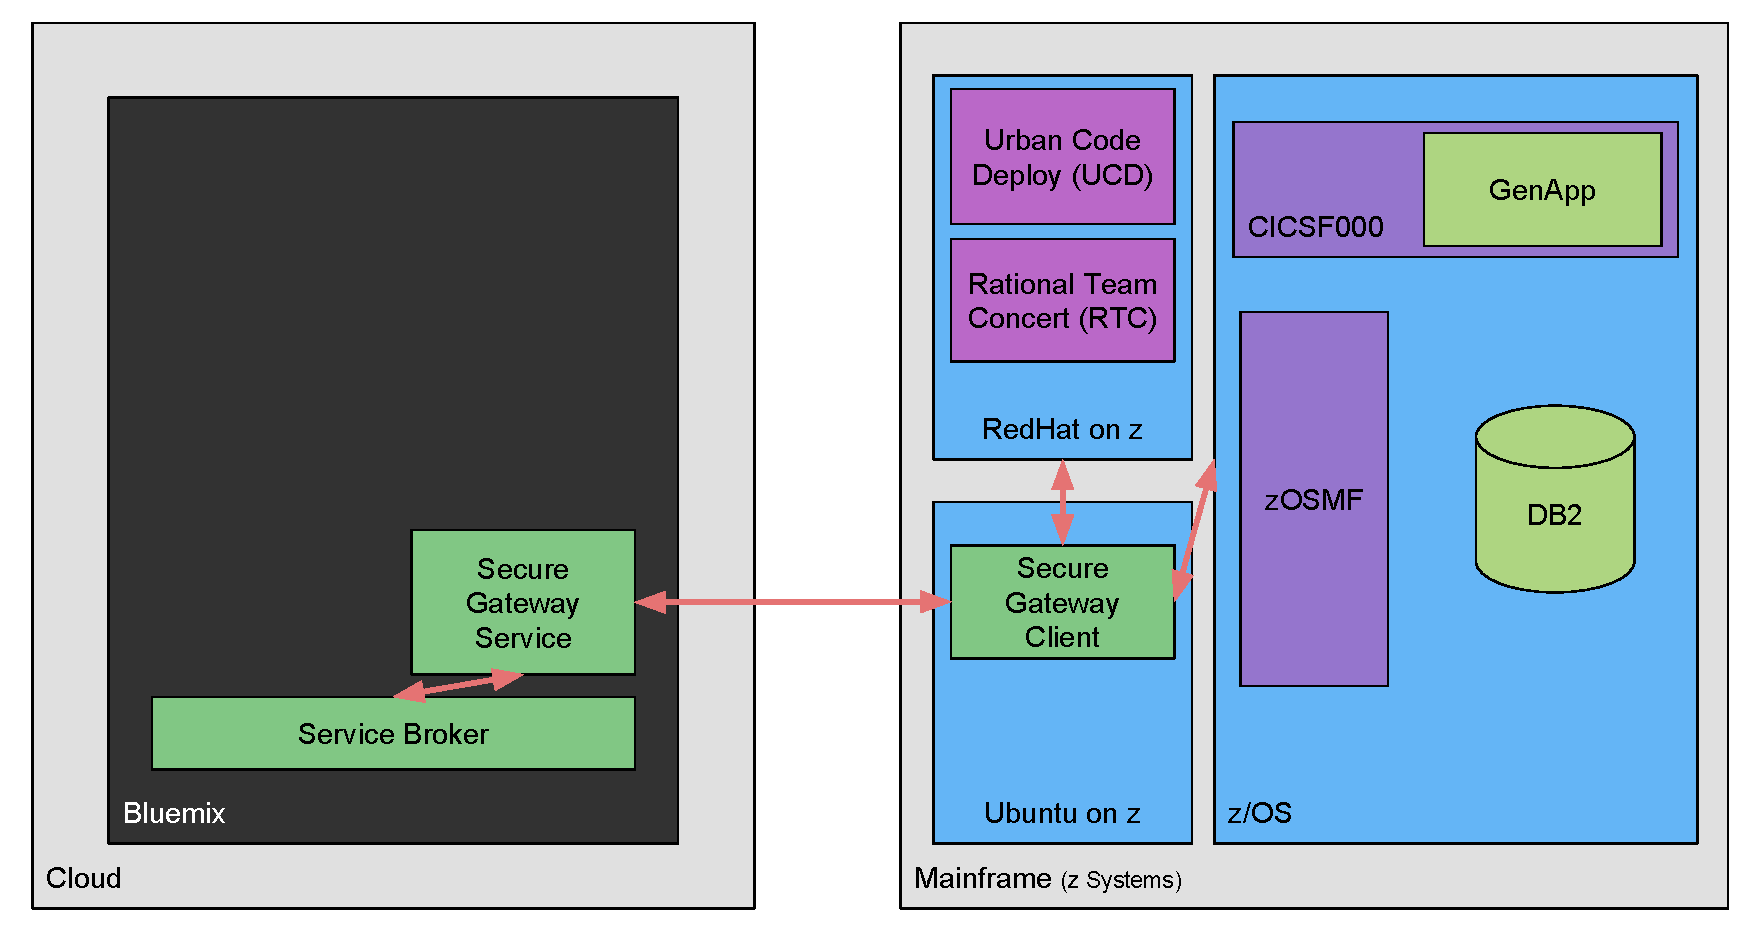
\includegraphics[scale=0.48]{images/kapitel_3/architektur_gesamt.pdf}
  \caption{Übersicht der Zielarchitektur}
  \label{fig:architektur_gesamt}
\end{figure}

\subsection{Erstellen eines Software Service Templates}
Damit CICS-Regionen automatisiert auf dem Mainframe erstellt werden können, muss ein Software Service Template (auch
Workflow genannt) in zOSMF angelegt werden. Dies kann anschließend wiederholt gestartet werden.

Um einen Workflow anzulegen wird das zOSMF in einem Webbrowser geöffnet und nach einem erfolgreichen Login erscheint auf der
linken Seite das Konfigurationsmenü (siehe dazu Abbildung \ref{fig:zosmf_uebersicht} auf Seite \pageref{fig:zosmf_uebersicht}).

\begin{figure}[h]
  \centering
    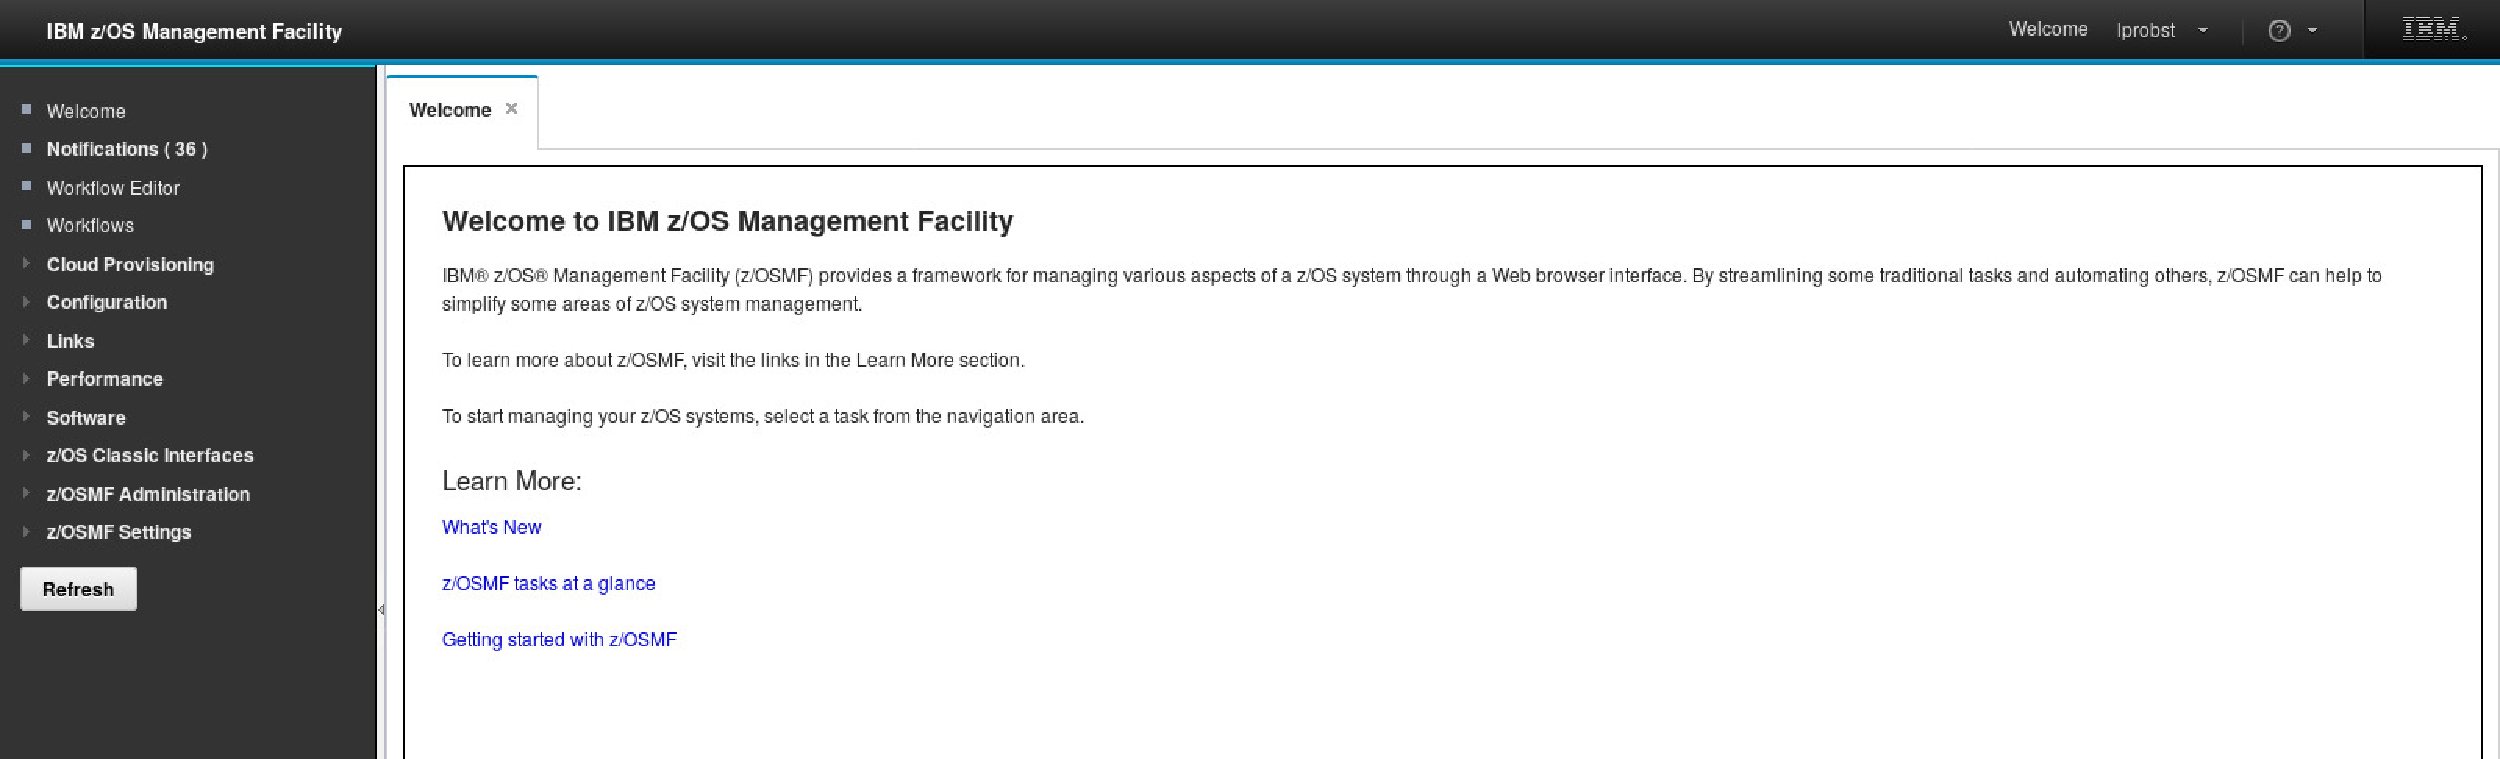
\includegraphics[scale=0.32]{images/kapitel_3/zosmf_uebersicht.pdf}
  \caption{Web-Interface von zOSMF}
  \label{fig:zosmf_uebersicht}
\end{figure}

Dort kann über den Menüpunkt \path{Cloud Provisioning} und anschließendem Klick auf \path{Software Service} die Übersicht
der CICS-Regionen angezeigt werden. Wie in Abbildung \ref{fig:zosmfsoftwareservice} auf Seite
\pageref{fig:zosmfsoftwareservice} zu sehen sind in diesem Beispiel derzeit sechs CICS-Regionen eingerichtet und drei
wurden gelöscht.

\begin{figure}[h]
  \centering
    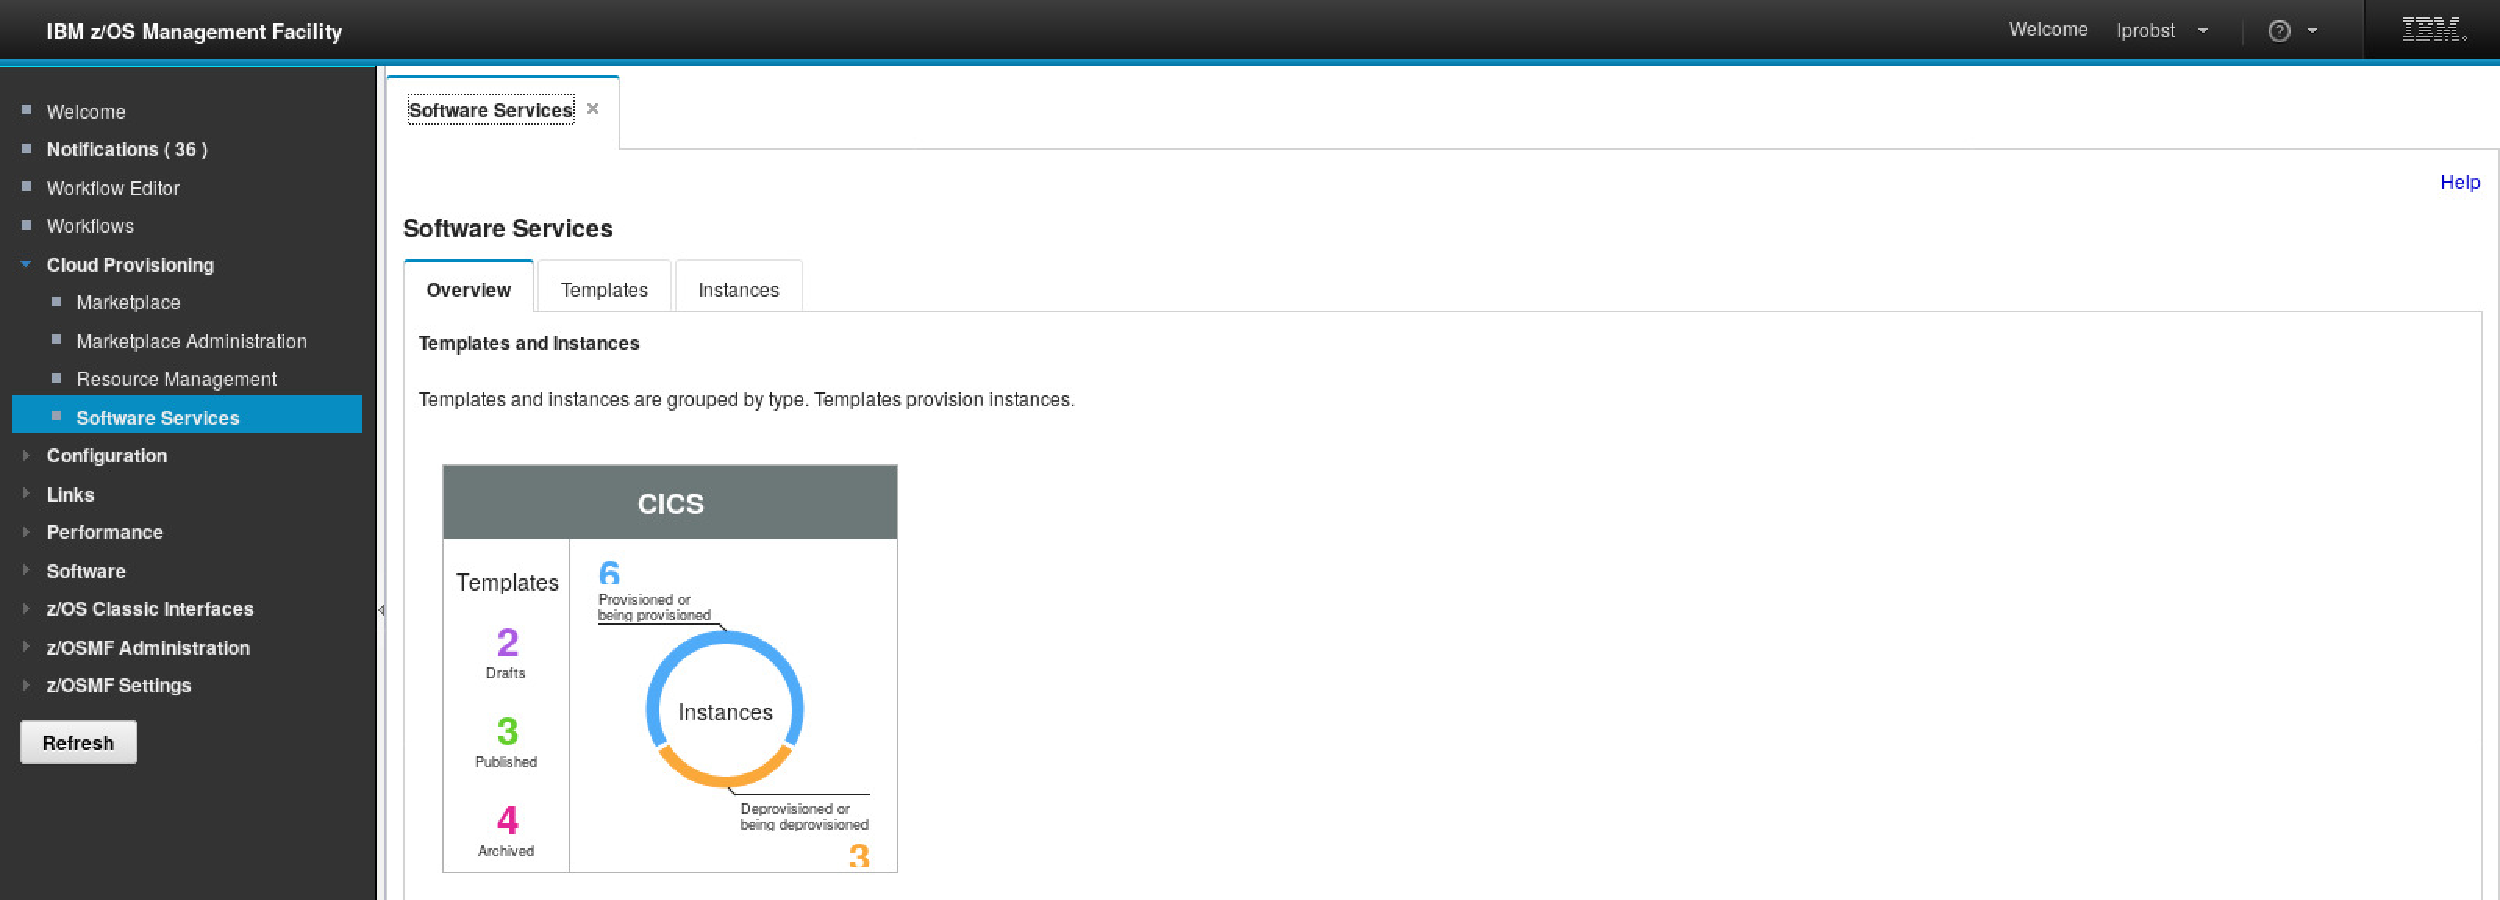
\includegraphics[scale=0.32]{images/kapitel_3/zosmf_softwareservice.pdf}
  \caption{Übersicht der CICS-Regionen}
  \label{fig:zosmfsoftwareservice}
\end{figure}

Über den Reiter \path{Templates} kann die Übersicht über alle angelegten Templates angezeigt werden. Über den Button
\path{Create} kann ein neues Software Service Template eingerichtet werden. Als Name wird hier
\path{cics53_mas_liberty_ucd} angegeben.

Dieser Workflow muss einerseits die CICS-Region in der CICS-Runtime hinzufügen und anmelden. Außerdem muss aus einem
vorgegebenen Pool an Port-Nummern eine ausgewählt und der CICS-Region konfiguriert werden.

Sobald die CICS-Region erfolgreich eingerichtet wurde, muss diese an dem UCD angemeldet werden, damit im späteren
Verlauf auch Anwendungen über UCD auf der Region installiert und eingerichtet werden können.

Nach der Speicherung des Templates wird dies in der Liste aller Templates angezeigt. Ein Klick auf dieses öffnet die
detaillierten Informationen darüber. Siehe dazu Abbildung \ref{fig:zosmftemplate} auf Seite \pageref{fig:zosmftemplate}.

\begin{figure}[h]
  \centering
    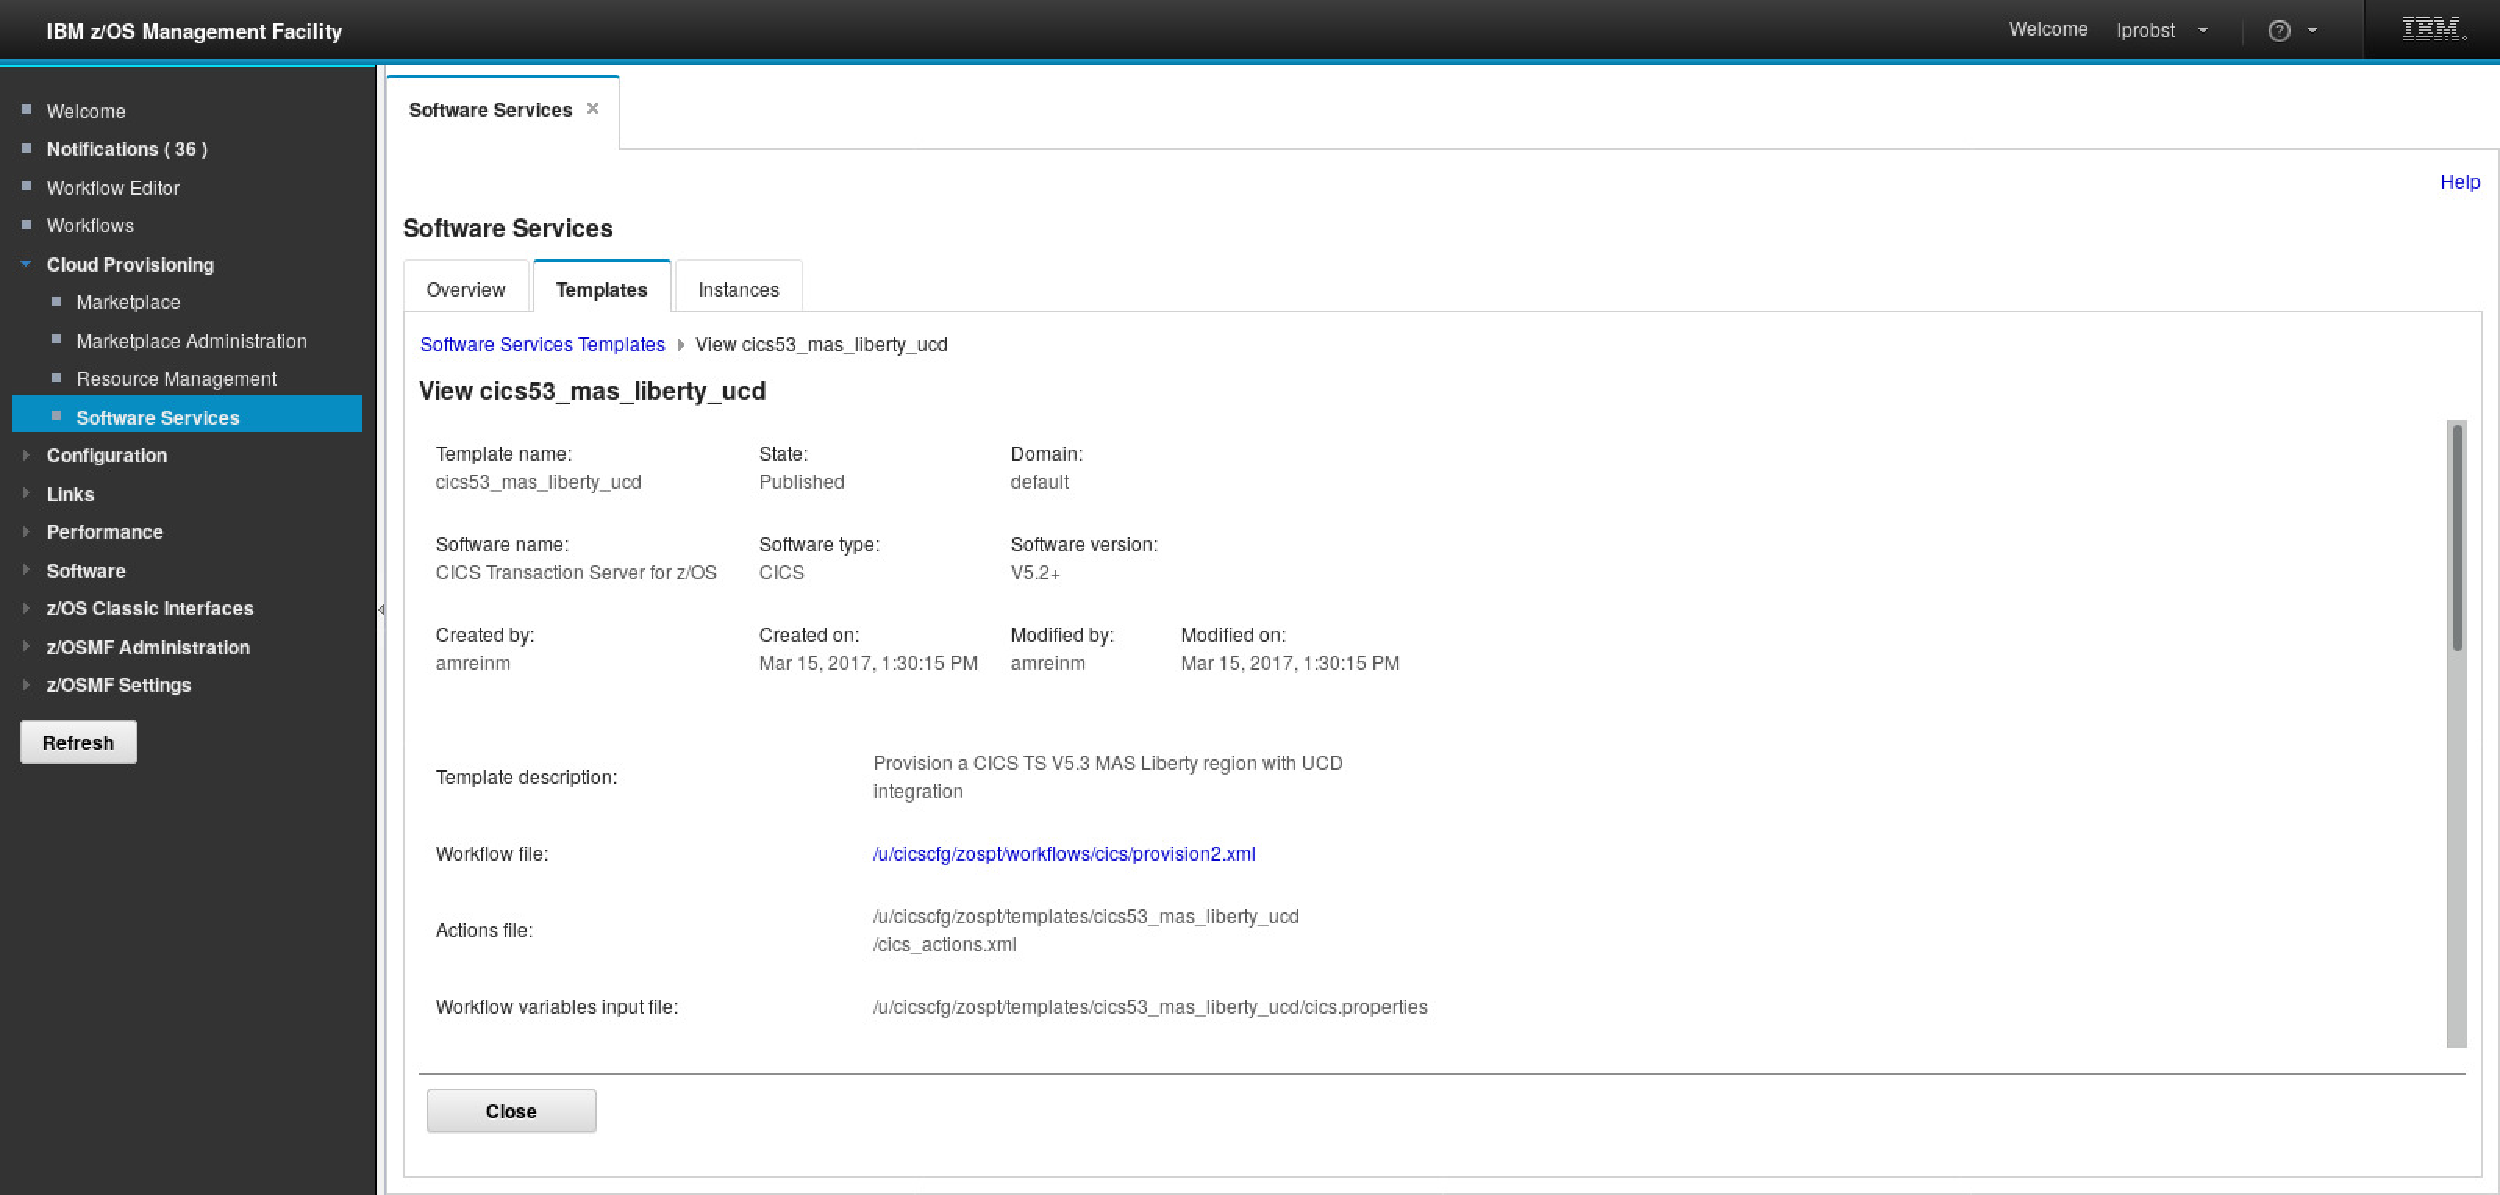
\includegraphics[scale=0.32]{images/kapitel_3/zosmf_template.pdf}
  \caption{Informationen des eingerichteten Software Service Templates}
  \label{fig:zosmftemplate}
\end{figure}

\subsection{RACF Profil einrichten}
Unter z/OS werden neben Identifikation und Verifikation von Benutzern und deren Protokollierung auch die Zugriffe
auf Resourcen über RACF Profile verwaltet. Diese implementieren die System Authorization Facility (kurz SAF) des Kernels
(MVS).

Um einem Benutzer oder einem Programm Zugriff auf Resourcen zu gewähren, müssen dafür RACF-Profile eingerichtet werden.

Für die Nutzung der zOSMF RESTFul-"-Schnittstelle müssen die in Listing \ref{RACF Profil einrichten} auf Seite
\pageref{RACF Profil einrichten} aufgeführten Kommandos ausgeführt werden.

Die Befehle werden als Administrator des Systems in die Kommandozeile (Terminal) eingegeben. Erst dann funktioniert die
RESTFul-Schnittstelle des zOSMF.

\begin{lstlisting}[language=bash, caption=RACF Profil einrichten, label=RACF Profil einrichten]
   $ RDEFINE ZMFAPLA IZUDFLT.REST.** UACC(NONE)
   $ PERMIT IZUDFLT.REST.** CLASS(ZMFAPLA) ID(IZUSVR) ACCESS(READ)
   $ SETROPTS RACLIST(ZMFAPLA) REFRESH
\end{lstlisting}

Ob die Einrichtung funktioniert hat, kann durch den Aufruf der RESTFul-Schnittstelle überprüft werden. Dazu werden z.B.
die Information der zOSMF Instanz durch die Schnittstelle abgerufen. Die URL ist die im Secure Gateway definierte mit der
Endung \path{/zosmf/info}. Die URL sollte wie folgt aussehen: \path{https://securegatewayUrl:securegatewayPort/zosmf/info}.

Alternativ kann im gleichen Netzwerk auch die IP-Adresse des Systems verwendet werden. Dann muss allerdings der Port
\path{60443} genutzt werden, da dies der Standardport für die Schnittstelle ist. In diesem Fall setzt sich die URL wie
folgt zusammen: \path{https://ipMainframe:60443/zosmf/info}.

\subsection{Einrichten des Secure Gateways}
\label{subsection:secureGateway}
Für die Kommunikation zwischen Bluemix (Cloud) und z System (Lokal) wird eine dauerhafte Verbindung benötigt. Die Umsetzung
erfolgt durch den Secure Gateway-Service von Bluemix. Dieser befindet sich im Bluemix-Katalog im Bereich \path{Integrate}.

Nach der Instanziierung des Services kann dieser angeklickt werden, wodurch sich die Konfigurationsansicht öffnet. Dort
befindet sich im Bereich \path{Verwalten} die Möglichkeit, ein neues Gateway hinzuzufügen. Dazu wird, nach einem Klick auf
das weiße \textit{Plus}, lediglich ein Name eingegeben. Ein Beispiel hierfür ist \path{Mainframe}.

Nun wird über den Tab \path{Clients} dem Gatway ein neuer Client hinzugefügt. In dem sich öffnenden Fenster wird die
Gateway-ID und der Sicherheitstoken für den neuen Client angezeigt. Diese müssen notiert werden, da sie nicht noch einmal
angezeigt werden können.

Anschließend wird der passende Client für die Systemarchitektur heruntergeladen und auf dem Zielsystem installiert.

\begin{lstlisting}[language=bash, caption=Secure Gateway für s390x installieren, label=Secure Gateway s390x installieren]
   $ wget https://sgmanager.ng.bluemix.net/installers/ibm-securegateway-client-1.7.1+client_s390x.deb
   $ sudo dpkg -i ibm-securegateway-client-1.7.1+client_s390x.deb
\end{lstlisting}

Während der Installation wird nach der notierten Gateway-ID und dem Sicherheitstoken gefragt. Nach erfolgreicher Installation
erscheint der neue Client in Bluemix im Reiter \path{Clients}.

Standardmäßig lässt der Secure Gateway nur Verbindungen zu, welche in einer ACL-Datei (Access Control List) aufgeführt sind.
Damit die Ubuntu-Maschine nun mit jeweils dem RedHat- und dem z/OS-System kommunizieren kann, wird im Ordner
\path{/opt/ibm/SecureGateway/client} eine Datei namens \path{ACL.txt} angelegt.

\begin{lstlisting}[language=bash, caption=ACL-Datei anlegen, label=ACL-Datei anlegen]
   $ cd /opt/ibm/SecureGateway/client
   $ touch ACL.txt
\end{lstlisting}

In der \path{ACL.txt}-Datei müssen nun die folgenden Zeilen eingefügt werden. Links vom Doppelpunkt werden die jeweiligen
lokalen IP-Adressen eingetragen, und nach dem Doppelpunkt können die Ports angegeben werden. Die Ports werden hier allerdings
nicht benötigt und deshalb leer gelassen. Die Verbindung zu den einzelnen Systemen soll hier nicht eingeschränkt werden.

\begin{lstlisting}[language=bash, caption=Inhalt der ACL-Datei, label=Inhalt der ACL-Datei]
   acl allow 10.3.20.47:
   acl allow 10.3.20.233:
\end{lstlisting}

Nun muss in der Konfigurationsdatei des installierten Clients die ACL.txt-Datei angegeben werden. Dazu wird im Ordner
\path{/etc/ibm/} die Datei \path{sgenvironment.conf} bearbeitet. In Zeile 18 muss der folgende Inhalt eingefügt werden:

\begin{lstlisting}[language=bash, numbers=left, firstnumber=18, caption=Konfigurationsdatei anpassen, label=Konfigurationsdatei anpassen]
   ACL_FILE=/opt/ibm/securegateway/client/ACL.txt
\end{lstlisting}

Damit können nun unter allen Ports Verbindungen zu den beiden Maschinen \path{10.3.20.47} und \path{10.3.20.233} aufgebaut
werden. Das ist wichtig, damit in Bluemix mehrere Routen (Ziele) definiert werden können.

Im Anschluss können nun Ziele für den installierten Gateway hinzugefügt werden. Ziele sind dabei immer Rechner, Programme
oder Schnittstellen im Netzwerk des Gateways, die in der \path{ACL.txt}-Datei angegeben wurden oder er selbst. Außerdem
können die Ports für die Verbindung angegeben werden.

Als erstes Ziel wird eine Verbindung zum zOSMF eingerichtet. Der Name hierfür ist \path{zOSMF}. Die IP-Adresse ist das
z/OS System mit \path{10.3.20.47} und der Port ist der der RESTFul-Schnittstelle von zOSMF mit \path{60443}. Als Protokoll
wird \path{https} ausgewählt.

Das zweite Ziel wird die Verbindung zu UCD repräsentieren. Dazu wird ein neues Ziel hinzugefügt und als Name \path{UCD}
und als IP-Adresse die des RedHat-Systems, \path{10.3.20.233}, eingetragen. Der Port der RESTFul-Schnittstelle von UCD
ist \path{8443}, und als Protokoll wird ebenfalls \path{https} ausgewählt.

Als letztes wird noch ein drittes Ziel - für den DB2 Service - hinzugefügt. Der Name ist dabei \path{DB Service}, die
IP-Adresse die des z/OS-Systems, welches die DB Instanz hält mit \path{10.3.20.47} und als Port der DB2 Service Port mit
\path{4740}.

Nun erstellt der Secure Gateway-Service in Bluemix drei individuelle Domains mit zugehörigen  Ports für die jeweiligen
Verbindungen. In diesem Fall ist dies \path{https://cap-sg-prd-1.integration.ibmcloud.com:16283} für das zOSMF-Interface,
\path{https://cap-sg-prd-1.integration.ibmcloud.com:15543} für die UCD Verbindung und als letzte Domain
\path{http://cap-sg-prd-1.integration.ibmcloud.com:16950} für den DB2 Service.

Da die URL mit dem Port auf die lokale IP des Mainframes mit dem zOSMF-Port gemappt wird, kann im Browser das zOSMF mit
der URL aufgerufen werden, ohne dass man sich im Netzwerk des Mainframes befinden muss. Das selbe gilt auch für UCD und
den DB2 Service.

Nun besteht eine Verbindung zwischen Bluemix und dem lokalem Mainframe, die ab sofort genutzt und beliebig erweitert
werden kann.

\subsection{Schreiben eines Service Brokers}
\label{subsection:writeservicebroker}
Da das zOSMF nun auch von außerhalb des lokalen Netzwerkes aufrufbar ist, kann nun der Service Broker entwickelt werden,
der die Ressourcen in Form von CICS-Regionen auf dem Mainframe bereitstellen soll. Dazu greift der Service Broker über den
Secure Gateway auf die RESTFul-Schnittstellen von zOSMF bzw. UCD zu.

Um einen Service Broker in Bluemix anbieten zu können, muss dieser in einem Container laufen und via URL aufrufbar sein.
In diesem Container läuft die Service Broker Anwendung, welche neben einem REST-Interface auch das Konfigurationsinterface
zur Verfügung stellt.

Das REST-Interface wird von einem Bluemix-Nutzer einmalig genutzt, um eine Service-Instanz zu erstellen, diese zu
konfigurieren oder zu löschen. Bei der Erstellung kann der Nutzer angeben, welchen \path{Plan} er nutzen möchte.

Mit dem Konfigurationsinterface kann jeder Benutzer individuell seinen instanziierten Service konfigurieren und erweitern.

Eine Übersicht über die Architektur eines Service Brokers ist in Abbildung \ref{fig:architektur_servicebroker} auf Seite
\pageref{fig:architektur_servicebroker} zu finden.

\begin{figure}[h]
  \centering
    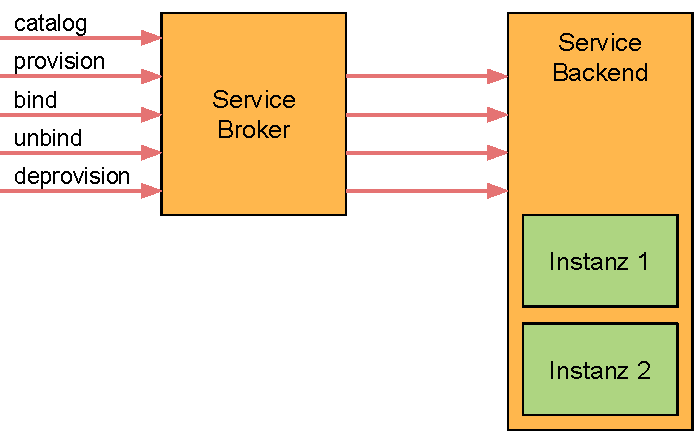
\includegraphics[scale=0.9]{images/kapitel_3/architektur_servicebroker.pdf}
  \caption{Allgemeine Architektur eines Service Brokers}
  \label{fig:architektur_servicebroker}
\end{figure}

In dieser Abbildung ist zu sehen, dass der Service Broker die Funktionen \path{catalog}, \path{provision}, \path{bind},
\path{unbind} und \path{deprovision} umsetzen muss.

Bei \path{catalog} wird der Katalog des Service Brokers zurückgegeben und der Nutzer kann sich diese anschauen.

Die Funktion \path{provision} ermöglicht die Instantiierung des Service Brokers in einer Bluemix Umgebung.

Bei \path{bind} handelt es sich um das Verbinden eines Services und einer Runtime um Daten über die VCAP-Variablen
auszutauschen.

\path{Unbind} löst eine schon geschaffene Verbindung wieder auf und \path{deprovision} löscht den instanziierten Service
Broker komplett aus dem eigenen Bluemix Bereich.

In dieser Arbeit wird der Service Broker in der Programmiersprache \path{Python}\footnote{https://www.python.org}
geschrieben. Dazu wird in Bluemix ein Python Cloud Foundry-Container aus der Katalog Kategorie
\path{Cloud Foundry-Anwendungen} erstellt.

Anschließend wird in der Übersicht, in der gerade erstellten Anwendung, im Bereich \path{Continuous Delivery} ein JazzHub
Git-Repository hinzugefügt. In diesem wird der Quellcode abgelegt und nach einem \path{push} durch Git ein automatischer
Buildprozess angestoßen, welcher den Service Broker bereitstellt.

Um mit der Entwicklung zu beginnen, wird zuallererst das Git-Repository auf den eigenen Rechner geklont. Dazu wird mit
Hilfe des \path{clone}-Befehls von Git dieses kopiert.

\begin{lstlisting}[language=bash, caption=Git-Repository Klonen, label=Git-Repository Klonen]
   $ git clone https://hub.jazz.net/benutzerName/anwendungsName
\end{lstlisting}

Dabei ist der Pfad \path{benutzerName} der Benutzername des Accounts, welcher den Cloud Foundry Container erstellt hat
und \path{anwendungsName} der Name des Containers. Die vollständige URL kann jedoch auch nach dem Ertellen des Repositorys
kopiert werden.

Wenn der Klonvorgang erfolgreich ist, wird auf dem Entwicklungsrechner ein Ordner mit dem Namen der Cloud Foundry
Anwendung erstellt, in welchem Beispieldaten für eine Python-Anwendung für Bluemix hinterlegt sind.

Nach der Analyse des Service Brokers und der Schnittstellen die dieser zur Verfügung stellen muss, kann dieser entwickelt
werden. Eine Dokumentation der zu implementierenden Schnittstellen ist in  Abbildung \ref{fig:swagger_servicebroker} auf
Seite \pageref{fig:swagger_servicebroker} zu sehen.

\begin{figure}[h]
  \centering
    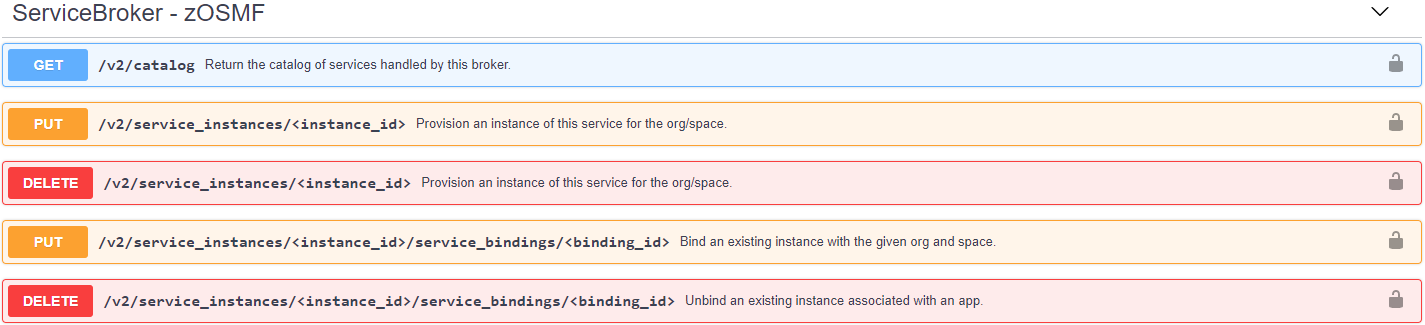
\includegraphics[scale=0.38]{images/kapitel_3/swagger_servicebroker.png}
  \caption{Schnittstellen des Service Brokers}
  \label{fig:swagger_servicebroker}
\end{figure}

Damit die Anwendung in Python geschrieben werden kann, werden drei Libraries benötigt. Diese werden in eine Datei mit
Namen \path{requirements.txt} gespeichert. Bei den Abhängigkeiten handelt es sich um \path{Flask}, \path{flask_basicauth}
und \path{uuid}.

\path{Flask} wird benötigt, um realtiv einfach ein REST-Interface in Pyhton bereit stellen zu können, welches über
mehrere Endpunkte verfügt.

Bei \path{flask_basicauth} handelt es sich um ein Plugin für Flask, welches es ermöglicht einzelne Routen über eine
Authentifizierung zu sichern. Das wird benötogt, da das erstellen einer Instanz des Service Brokers laut Definition eine
Authentifizierung vorsieht.

Mit \path{uuid} können einmalige Identifikatoren erstellt werden, welche jede Instanz des Service Brokers eindeutig
identifizieren können. Auch diese Eigenschaft wird laut Definition eines Service Brokers benötigt.

Wenn die Cloud Foundry-Runtime nach einem Upload der Daten gebaut wird, werden automatisch alle Abhängigkeiten, welche
in der \path{requirements}-Datei angegeben sind, heruntergeladen und bereitgestellt.

Anschließend wird in der \path{runtime.txt}-Datei angegeben, in welcher Python-Version die Anwendung laufen soll. In diesem
Beispiel wird \path{python-3.5.1} genutzt.

Auch hier kümmert sich die Cloud Foundry-Runtime automatisch um die Bereitstellung der geforderten Version der Runtime.

Damit Pyhton wissen kann um welche art der Anwendung es sich handelt, wird in der \path{Procfile}-Datei angegeben, wie
die Anwendung gestartet werden und welche Datei beim Start ausgeführt werden soll. Der Inhalt der Datei ist
\path{web: python app/main.py}. Dadurch wird definiert, dass es sich um eine \textit{web}-Anwendung handelt und die Datei
\textit{main.py} im Verzeichnis \textit{app} ausgeführt werden soll. Dies ist auch die einzige Python-Datei in dem
Projekt.

Im Verzeichnis \path{/app} gibt es nun mehrere Unterverzeichnisse und eine Datei.

Im \path{/app/templates}-Ordner wird das Template hinterlegt, welches der Nutzer sieht wenn er den Service instanziiert
hat und ihn nun konfigurieren möchte, das Dashboard.

Im \path{/app/static} Verzeichnis sind Ordner und Dateien die für die Darstellung des Dashbaords wichtig sind. Dort wird
das eigentliche Design und der Aufbau des Dashboards erstellt.

In der \path{app/main.py}-Datei werden unter anderem der Benutzername und das Passwort zum Erstellen einer Instanz definiert
und die Pläne die es für den Service geben soll.

Außerdem werden in der unteren Hälfte die REST-Endpunkte zum instanziiere, editieren, binden und löschen eines Service
Brokers für den Nutzer definiert. Diese sind von Cloud Foundry vorgegeben und müssen lediglich implementiert werden.
Bluemix kümmert sich beim instanziieren des Service Brokers um den richtigen Aufruf des Interfaces.

Nach der Entwicklung des Service Brokers können die Änderungen am Quellcode mit dem Git-Befehl \path{commit} gespeichert
werden. Hinter dem Parameter \path{m} kann eine Nachricht angegeben werden, welche die Änderung beschreibt.

\begin{lstlisting}[language=bash, caption=Änderungen speichern, label=Änderungen speichern]
   $ git commit -m "Update all files"
\end{lstlisting}

Anschließend können mit \path{push} alle gespeicherten Änderungen an das Git-Repository übertragen werden.

\begin{lstlisting}[language=bash, caption=Änderungen hochladen, label=Änderungen hochladen]
   $ git push
\end{lstlisting}

Der Continous Deployment Service, welcher automatisch mit dem Hinzufügen eines Git-Repositorys zu einer Anwendung
hinzugefügt wird, registirert den \path{push} in das Repository und baut ein neues Artefakt, welches in den Cloud Foundry
Container geladen und bereitgestellt wird.

Das Dashboard des entwickelten Service Brokers ist in Abbildung \ref{fig:servicebroker_oberflaeche} auf Seite
\pageref{fig:servicebroker_oberflaeche} zu sehen und der komplette Quellcode ist im öffentlichen
GitHub-\-Repository\footnote{https://github.com/Alienuser/ServiceBroker-zOSMF} hinterlegt.

\begin{figure}[h]
  \centering
    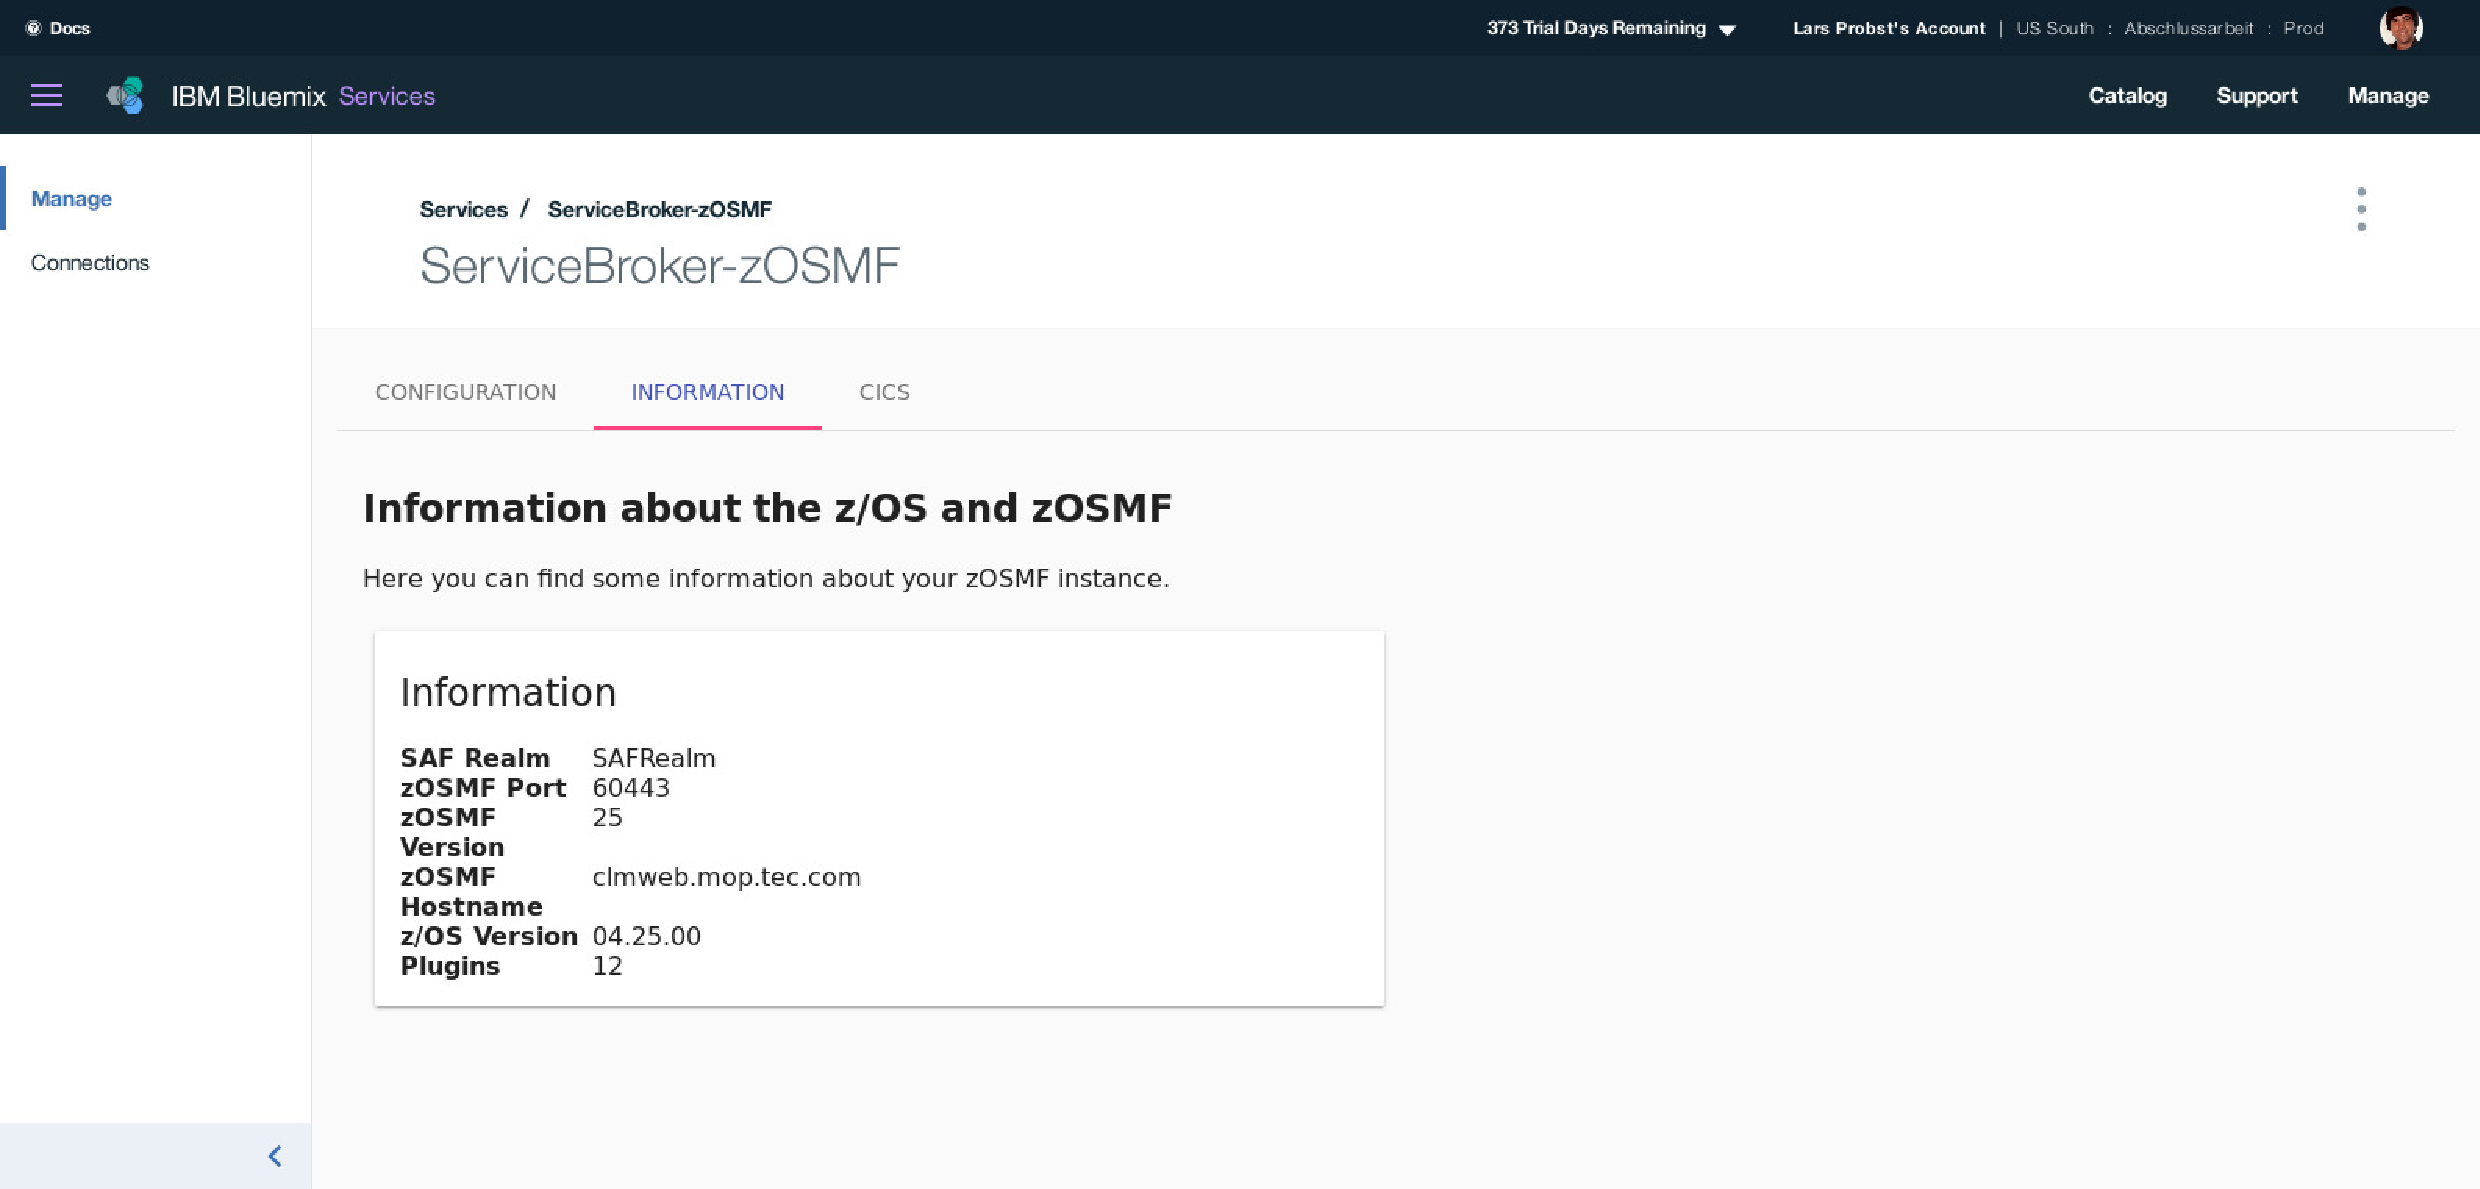
\includegraphics[scale=0.31]{images/kapitel_3/servicebroker_oberflaeche.pdf}
  \caption{Web-Interface des Service Brokers}
  \label{fig:servicebroker_oberflaeche}
\end{figure}

Nun läuft der Service Broker in einem Cloud Foundry Container und verfügt über eine eindeutige URL, über die er aufgerufen
werden kann. Dies ist für die weiteren Schritte wichtig.

Eine Übersicht über alle wichtigen Funktionen der RESTFul-Schnittstelle von zOSMF ist auf der
Hilfeseite\footnote{https://www.ibm.com/support/knowledgecenter/SSLTBW\_2.2.0/RESTServices.htm} zu finden.

\subsection{Instanziieren des Service Brokers}
Der geschriebene Service Broker, welcher nun unter Bluemix als Cloud Foundry-Applikation läuft, kann nun als Service
instanziiert werden.

Da die Anwendung in Bluemix Public läuft, kann der Service Broker nur als \path{Space Scoped} Broker hinzugefügt
werden, vergleiche dazu Kapitel \ref{sub:scopes} auf Seite \pageref{sub:scopes}.

Um den Service Broker in die eigene Organisation hinzuzufügen, muss zuallererst die Cloud Foundry CLI mit dem eigenen
Bluemix-Account und der Zielorganisation verbunden werden. Dazu wird im Terminal der \path{api}-Befehl ausgeführt.

\begin{lstlisting}[language=bash, caption=Definieren der API über die Cloud Foundry CLI, label=Definieren der API über die Cloud Foundry CLI]
   $ cf api api.ng.bluemix.net
\end{lstlisting}

Nun ist die Cloud Foundry CLI mit der amerikanischen Instanz von Bluemix verbunden, in die man sich nun mittels
\path{login} einloggen kann.

\begin{lstlisting}[language=bash, caption=Einloggen über die Cloud Foundry CLI, label=Einloggen über die Cloud Foundry CLI]
   $ cf login
\end{lstlisting}

Im Folgenden wird nach der E-Mail-Adresse und dem dazugehörigen Passwort des Bluemix-Accounts gefragt. Nach korrekter
Eingabe der Daten wird nach der Organisation gefragt, mit welcher das CLI verbunden werden soll.

Nach Eingabe der entsprechenden Zahl ist die Cloud Foundry CLI erfolgreich mit der Zielorganisation verbunden, und der
Service Broker kann dieser hinzugefügt werden.

Sollten in der Organisation mehrere Bereiche vorhanden sein, wird im Anschluss noch nach einer entsprechenden Auswahl
gefragt. Dabei ist egal, welcher Bereich ausgewählt wird, da der Service Broker in der kompletten Organisation zur Verfügung
steht.

Nun kann der Service Broker in die Organisation hinzugefügt werden. Dies geschieht über den Befehl \path{create-service-broker}.

\begin{lstlisting}[language=bash, caption=Service Broker einrichten, label=Service Broker einrichten]
   $ cf create-service-broker brokerName username password brokerURL --space-scoped
\end{lstlisting}

Dabei ist \path{brokerName} der Name des in Kapitel \ref{subsection:writeservicebroker} auf Seite
\pageref{subsection:writeservicebroker} angelegten Service Brokers.

Die Parameter \path{username} und \path{password} sind nicht die des Bluemix-Benutzerkontos, sondern die für den Zugriff
auf den Service Broker.

Die \path{brokerURL} ist die URL der Cloud Foundry-Applikation, in der der Service Broker aufrufbar ist.

Der letzte Parameter \path{--space-scoped} ist wichtig, da damit der Scope des Service Brokers angegeben wird. Wird dieser
bei der Nutzung von Bluemix Public weggelassen, erscheint eine Fehlermeldung.

Nach der Eingabe des Befehls sollte eine Information erscheinen, welche das erfolgreiche Hinzufügen des Service Brokers
quittiert.

Über die Cloud Foundry CLI gibt es zwei Möglichkeiten die aktuellen Services einzusehen, die für den Benutzer in der
Organisation zur Verfügung stehen. Der Befehl \path{marketplace} listet \textbf{alle} verfügbaren Services auf.

\begin{lstlisting}[language=bash, caption=Auflisten aller verfügbaren Services, label=Auflisten aller verfügbaren Services]
   $ cf marketplace
\end{lstlisting}

Wohingegen der \path{service-brokers}-Befehl nur die selbst (oder von einem eingeladenen Account) hinzugefügten Service
Broker auflistet.

\begin{lstlisting}[language=bash, caption=Auflisten aller Service Broker, label=Auflisten aller Service Broker]
   $ cf service-brokers
\end{lstlisting}

\subsection{Provisionieren des Service Brokers}
Da der Service Broker nun als solcher in der Bluemix Organisation eingerichtet wurde, kann eine Instanz des Services
für einen Bereich (Space) provisioniert werden.

Jeder Service kann nur in einem Bluemix-Bereich provisioniert werden. Für die kommenden Schritte ist es wichtig,
dass der richtige Bereich in der Cloud Foundry CLI ausgewählt ist. Über den \path{target}-Befehl kann der Bereich
neu definiert werden.

\begin{lstlisting}[language=bash, caption=Bereich (Space) in Cloud Foundry CLI wechseln, label=Bereich (Space) in Cloud Foundry CLI wechseln]
   $ cf target -s spaceName
\end{lstlisting}

Der Parameter \path{spaceName} gibt den Bereich an, der ausgewählt werden soll.

Die Provisionierung eines Services geschieht über den \path{create-service}-Befehl der Cloud Foundry CLI.

\begin{lstlisting}[language=bash, caption=Provisionieren eines Services, label=Provisionieren eines Services]
   $ cf create-service service servicePlan serviceName
\end{lstlisting}

Der Parameter \path{service} gibt den Service Broker an, welcher provisioniert werden soll. Das ist der \path{brokerName}-
Parameter aus Listing \ref{Service Broker einrichten} auf Seite \pageref{Service Broker einrichten}.

Der \path{servicePlan} gibt den Plan an, welcher genutzt werden soll. Zur Auswahl stehen die im Service Broker
konfigurierten.

Als letztes wird über \path{serviceName} ein Name vergeben, wie der Service in Bluemix genannt werden soll. Über diesen
wird er im Bluemix Dashboard angezeigt. Über den Namen kann er später auch verändert oder gelöscht werden. In diesem Beispiel
wird der Service Borker \path{Service Broker zOSMF} genannt.

Nun kann der provisionierte Service mit dem vergebenen Namen im Bluemix Dashbaord in der entsprechenden Organisation und
dem Bereich eingesehen werden. Ein Klick auf den Service öffnet die Informationsseite des Services.

\subsection{Nutzen des Service Brokers}
Da der Service Broker nun instanziiert ist, kann er in Bluemix genutzt werden. Folgend wird der Service Broker kurz
eingerichtet und die wichtigsten Optionen erklärt.

Dazu wird dieser aus dem Bluemix Dashboard geöffnet. Es erscheint die Ansicht der Konfiguration wie in Abbildung
\ref{fig:servicebroker_configuration} auf Seite \pageref{fig:servicebroker_configuration} zu sehen.

\begin{figure}[h]
  \centering
    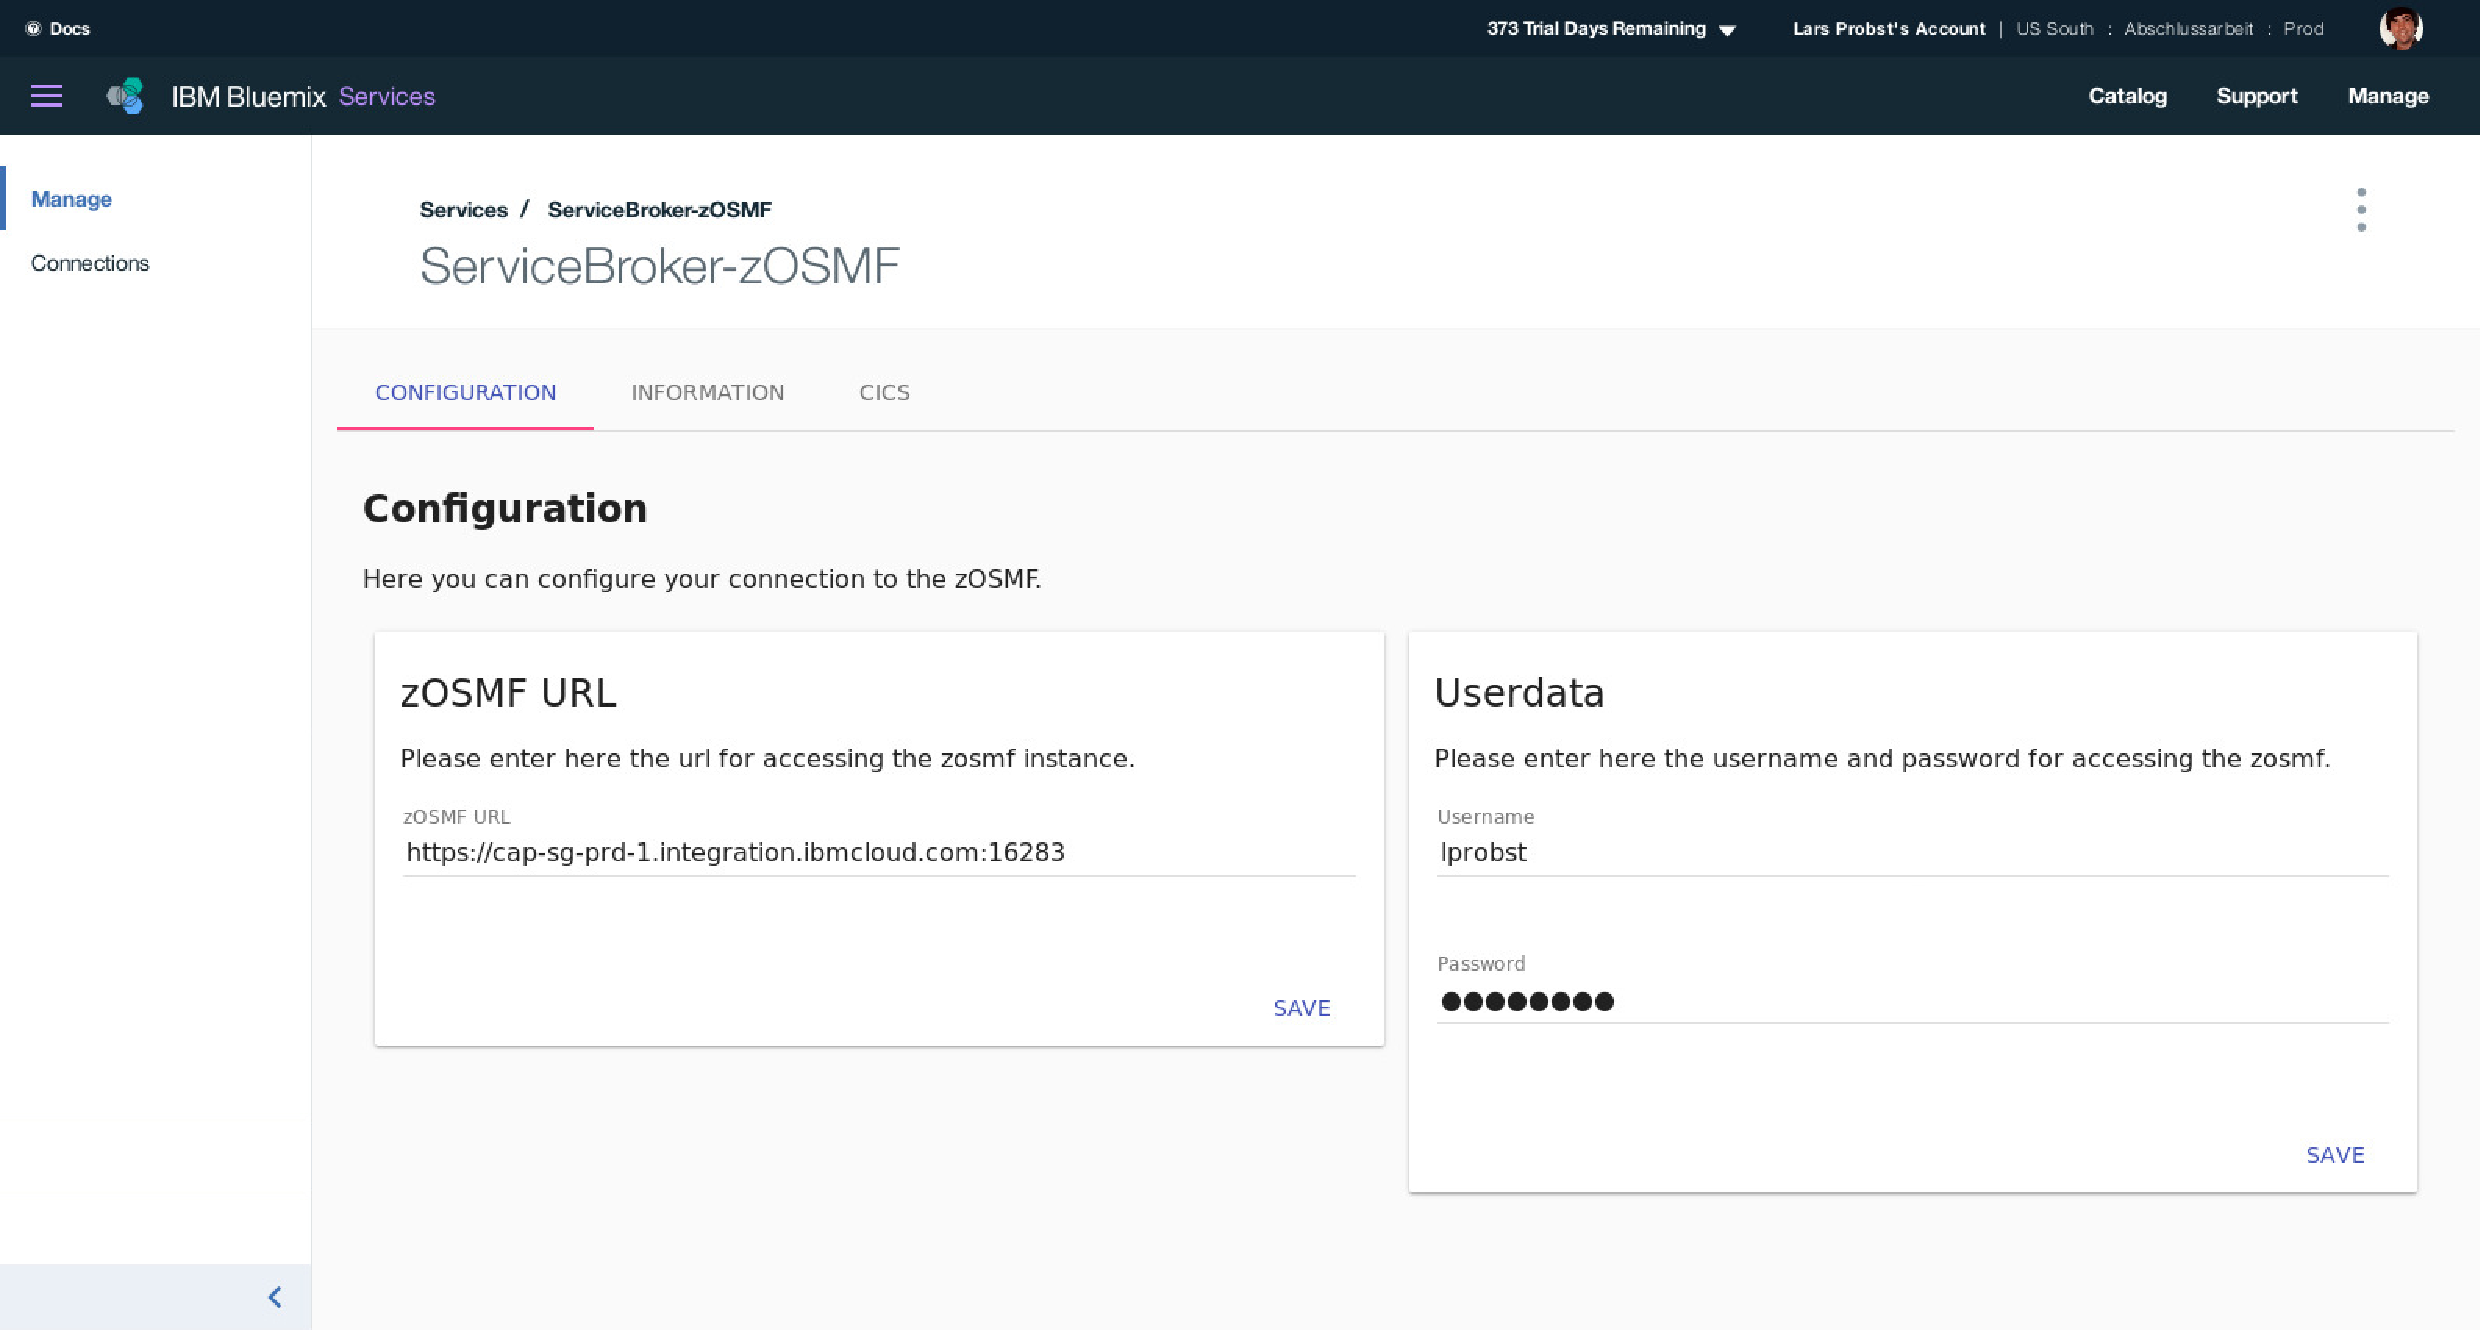
\includegraphics[scale=0.31]{images/kapitel_3/servicebroker_configuration.pdf}
  \caption{Konfiguration des Service Brokers}
  \label{fig:servicebroker_configuration}
\end{figure}

Dort wird im Bereich \path{zOSMF URL} die URL der zOSMF Instanz eingetragen, die im Secure Gateway hinterlegt ist. Dies
ist wichtig, damit der Service Broker das RESTFul-Interface aufrufen kann.

Damit der Service Broker Jobs in zOSMF ausführen kann, muss dieser sich am Interface authentifizieren. Dazu wird im Bereich
\path{Userdata} der Benutzername und das zugehörige Passwort eines zOSMF-Benutzers eingetragen, welcher über genügend
Rechte verfügt um Service Templates auszuführen.

Mit jeweils einem Klick auf \path{Save}, werden die Informationen dauerhaft im Service Broker gespeichert. Nun kann
getestet werden, ob die Eingabe der Daten korrekt war. Dazu wird der Reiter \path{Information} geöffnet. Dort sollten nun
Informationen über die zOSMF Instanz sowie der z/OS Version angezeigt werden.

Über den Reiter \path{CICS} können alle CICS-Regionen angezeigt, gestoppt oder gestartet werden oder auch neue
hinzugefügt werden. Außerdem können, nach einem Klick auf eine CICS-Runtime, Informationen über diese angezeigt werden.

Die Einrichtung des Service Brokers ist somit abgeschlossen und die wichtigsten Informationen sind bekannt.

\subsection{Einrichten der Toolchain}
\label{subsec:einrichten_der_toolchain}
Der Service Broker ist nun eingerichtet und somit können CICS-Regionen auf dem Mainframe bereitgestellt werden. Im folgenden
soll eine Toolchain in Bluemix eingerichtet werden, die es dem Entwickler ermöglicht, aus der Cloud heraus eine Anwendung
auf eine CICS-Region zu installieren.

Dazu wird das Dashboard von Bluemix geöffnet und anschließend über das Menü am linken oberen Rand der Punkt \path{Services}
und anschließend \path{DevOps} ausgewählt. Nun öffnet sich der Bluemix Bereich DevOps. In diesem ist es neben der Verwaltung
von Toolchains möglich, \textit{Pipelines} und \textit{Services} einzurichten.

Mit einem Klick auf \path{Toolchains} öffnet sich die Konfiguration dieser. Dort kann mit dem Button
\path{Toolchain erstellen} eine neue erstellt werden. Im sich öffnenden Fenster kann entweder eine Vorlage der zahlreichen
vorkonfigurierten Toolchains genutzt, oder eine eigene erstellt werden.

In diesem Beispiel wird die Vorlage mit dem Namen \path{Einfache Cloud Foundry-Toolchain (v2)} genutzt, da so ein
Git-Repository mitangelegt wird. Durch die Auswahl der Vorlage gelangt man in die Konfigurationsansicht. Siehe dazu
Abbildung \ref{fig:toolchain_konfiguration} auf Seite \pageref{fig:toolchain_konfiguration}.

\begin{figure}[h]
  \centering
    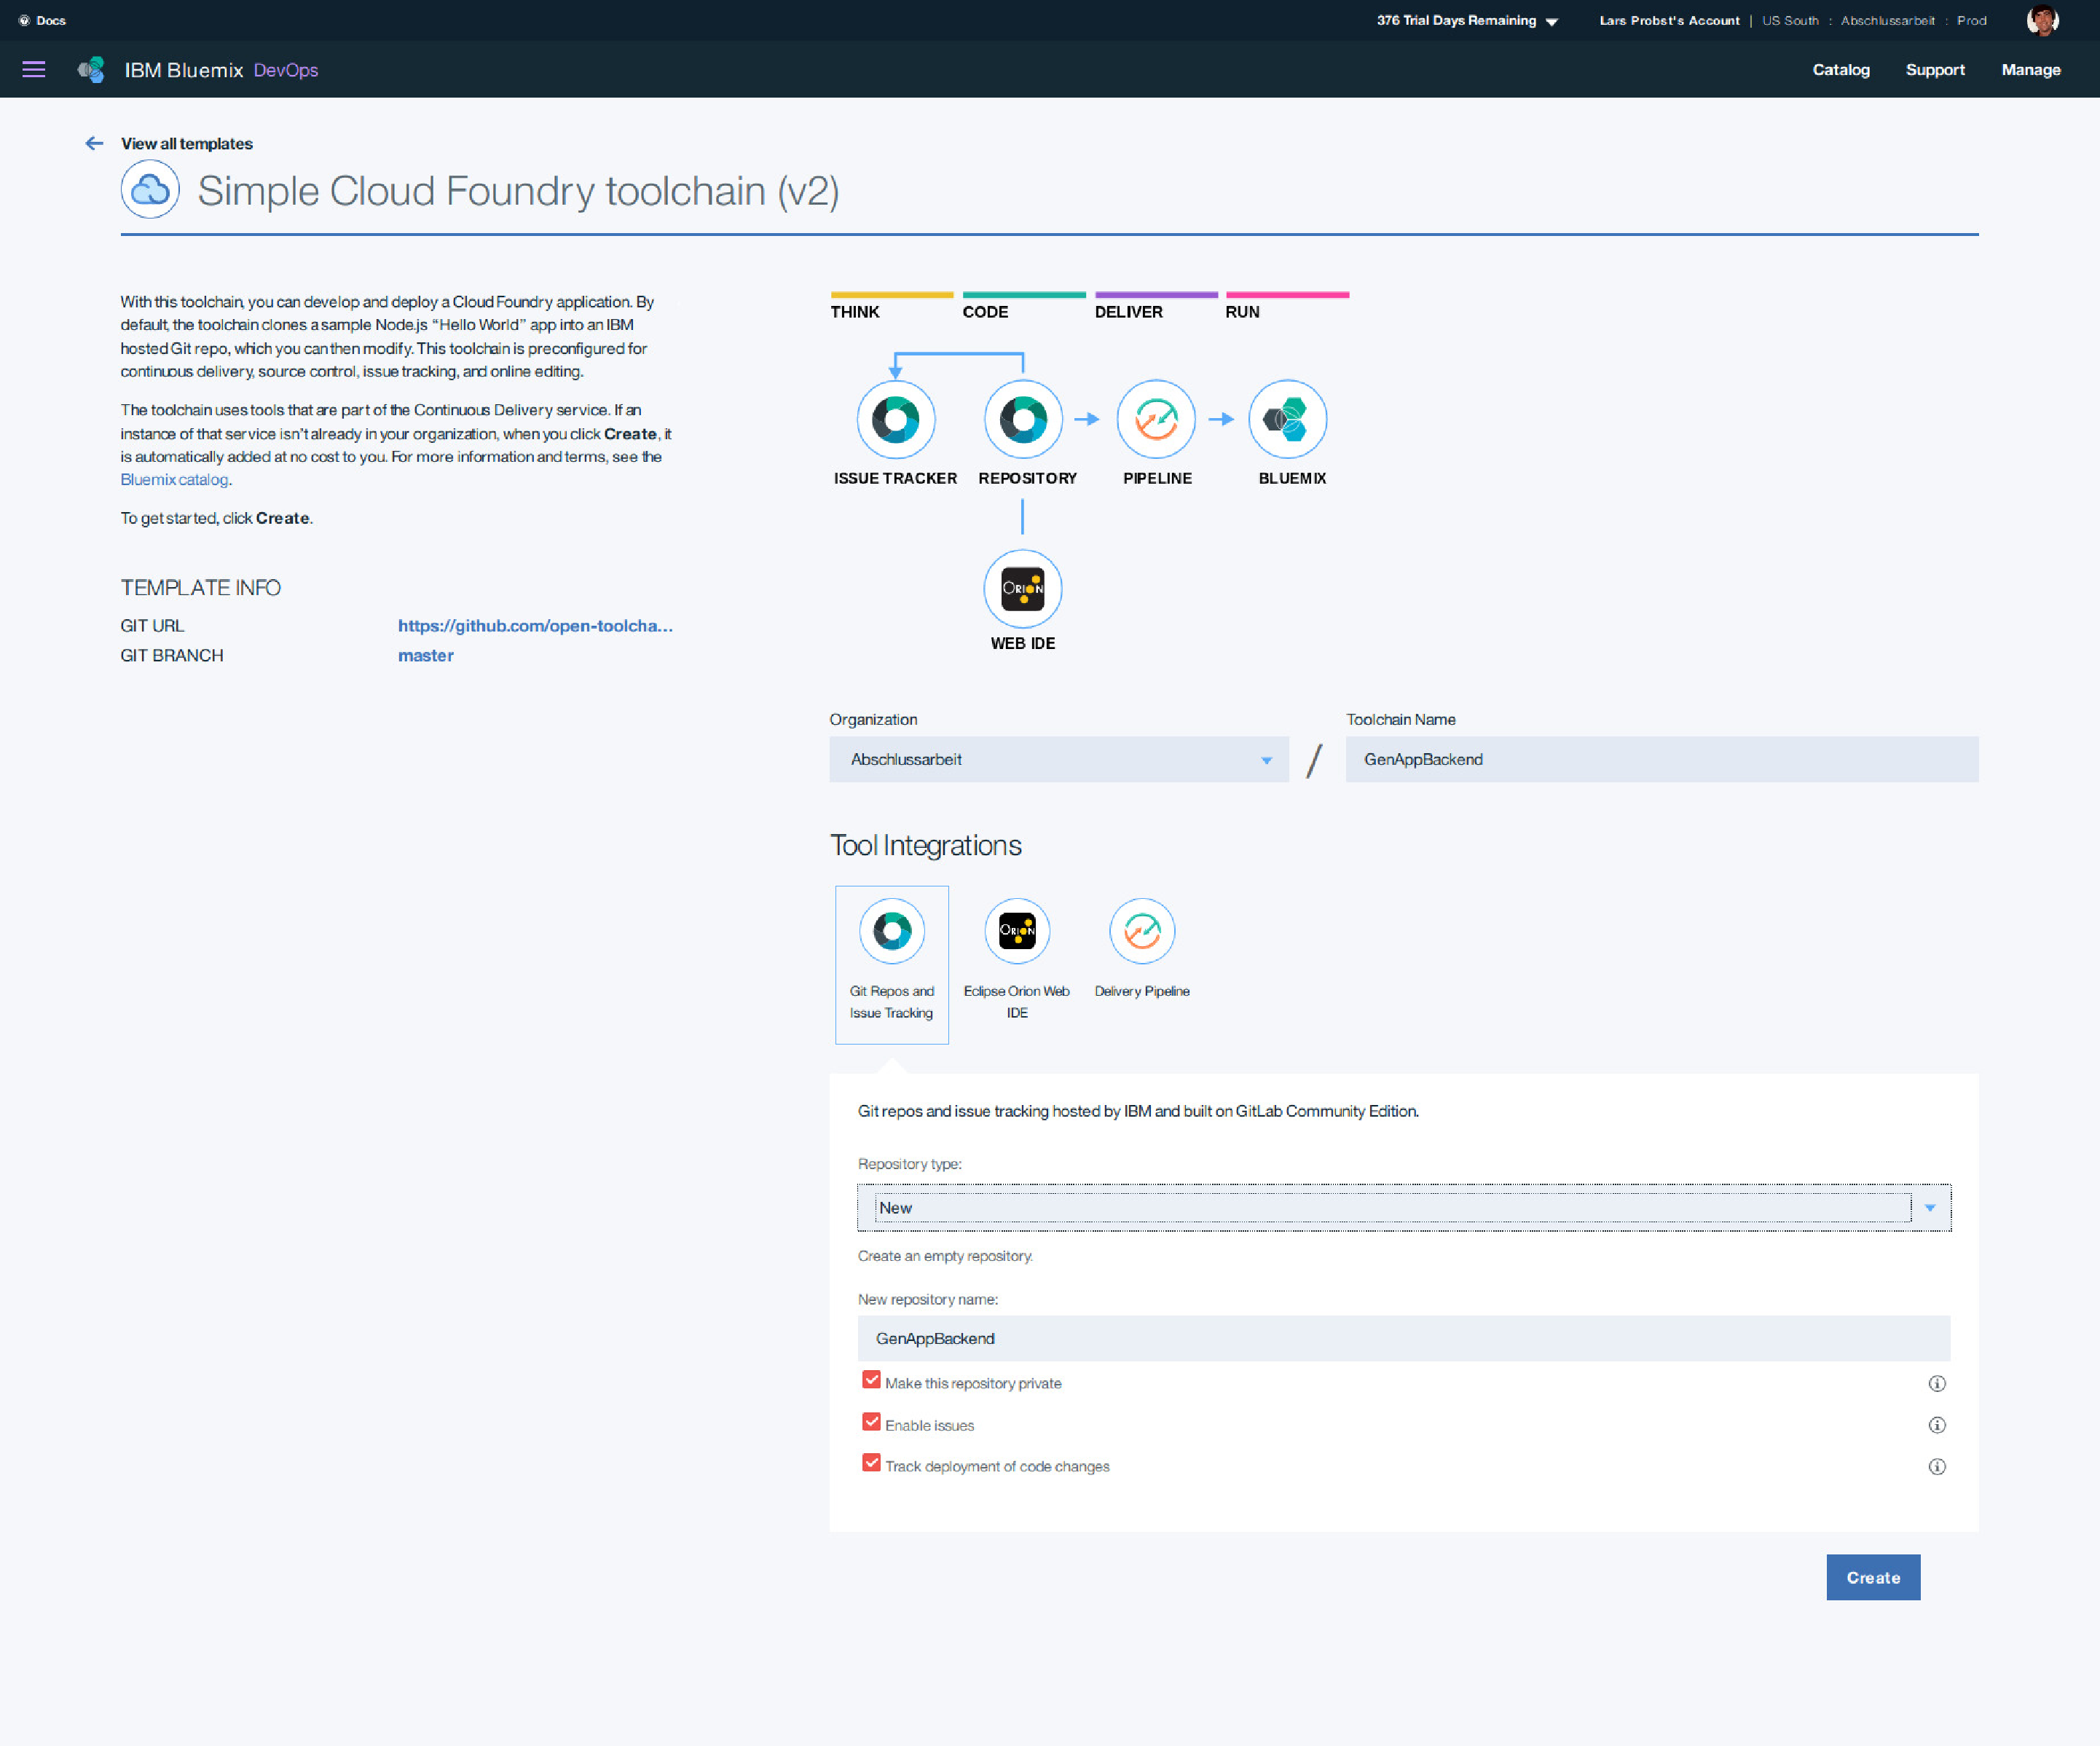
\includegraphics[scale=0.28]{images/kapitel_3/toolchain_konfiguration.pdf}
  \caption{Konfiguration der Toolchain}
  \label{fig:toolchain_konfiguration}
\end{figure}

Wie in der Abbildung zu sehen wurde als \textit{Repository type} \path{New} ausgewählt, damit ein neues, leeres
Git-Repositroy angelegt wird, in das der Quellcode gepushed werden kann. Außerdem wurde das Repository als \path{Private}
markiert und der Name \path{GenAppBackend} gewählt.

Über \path{Create} wird die Toolchain angelegt und steht ab sofort zur Verfügung. Allerdings ist diese noch nicht mit dem
Mainframe oder einer CICS-Region verbunden.

Im Anschluss öffnet sich die Übersicht der eingerichteten Toolchain. Dort kann das Git-Repository verwaltet, die
Web-IDE genutzt oder die Build Pipeline verwaltet werden.

Da es aktuell noch nicht möglich ist, direkt einen Mainframe oder eine CICS-Region über den Secure Gateway anzugeben und
keine eigenen Services zur Toolchain hinzugefügt werden können, muss diese Verbindung und die Installation des Artefaktes
noch händisch gemacht werden. Siehe mehr dazu im Kapitel \textit{Ausblick} \ref{sec:erweiterung_der_toolchain} auf Seite
\pageref{sec:erweiterung_der_toolchain}.

Die Einrichtung der Toolchain ist hiermit vorerst beendet, da die \path{DEPLOY}-Stage für jede CICS-Region anders
konfiguriert werden muss. Mehr dazu in Kapitel \ref{cha:prototypische_anwendung}, bei der Umsetzung der prototypischen
Anwendung.

\subsection{Einrichten von UCD}
Mit der Einrichtung der Toolchain in Kapitel \ref{subsec:einrichten_der_toolchain} auf Seite
\pageref{subsec:einrichten_der_toolchain} ist eine der zwei benötigten Funktionen umgesetzt, ein Artefakt aus dem Quellcode
zu bauen und auf dem Mainframe zu installieren.

Die zweite Funktion, die Installation über UCD, soll in diesem Kapitel beschrieben werden. Der Workflow des Software
Service Templates in zOSMF, der CICS-Regionen registriert, fügt diese nach erfolgreicher Einrichtung automatisch direkt
in UCD ein. Dies hat zur Folge, dass der Aufruf von UCD eine Übersicht aller eingerichteten CICS-Regionen anzeigt. Siehe
dazu Abbildung \ref{fig:ucd_overview} auf Seite \pageref{fig:ucd_overview}.

\begin{figure}[h]
  \centering
    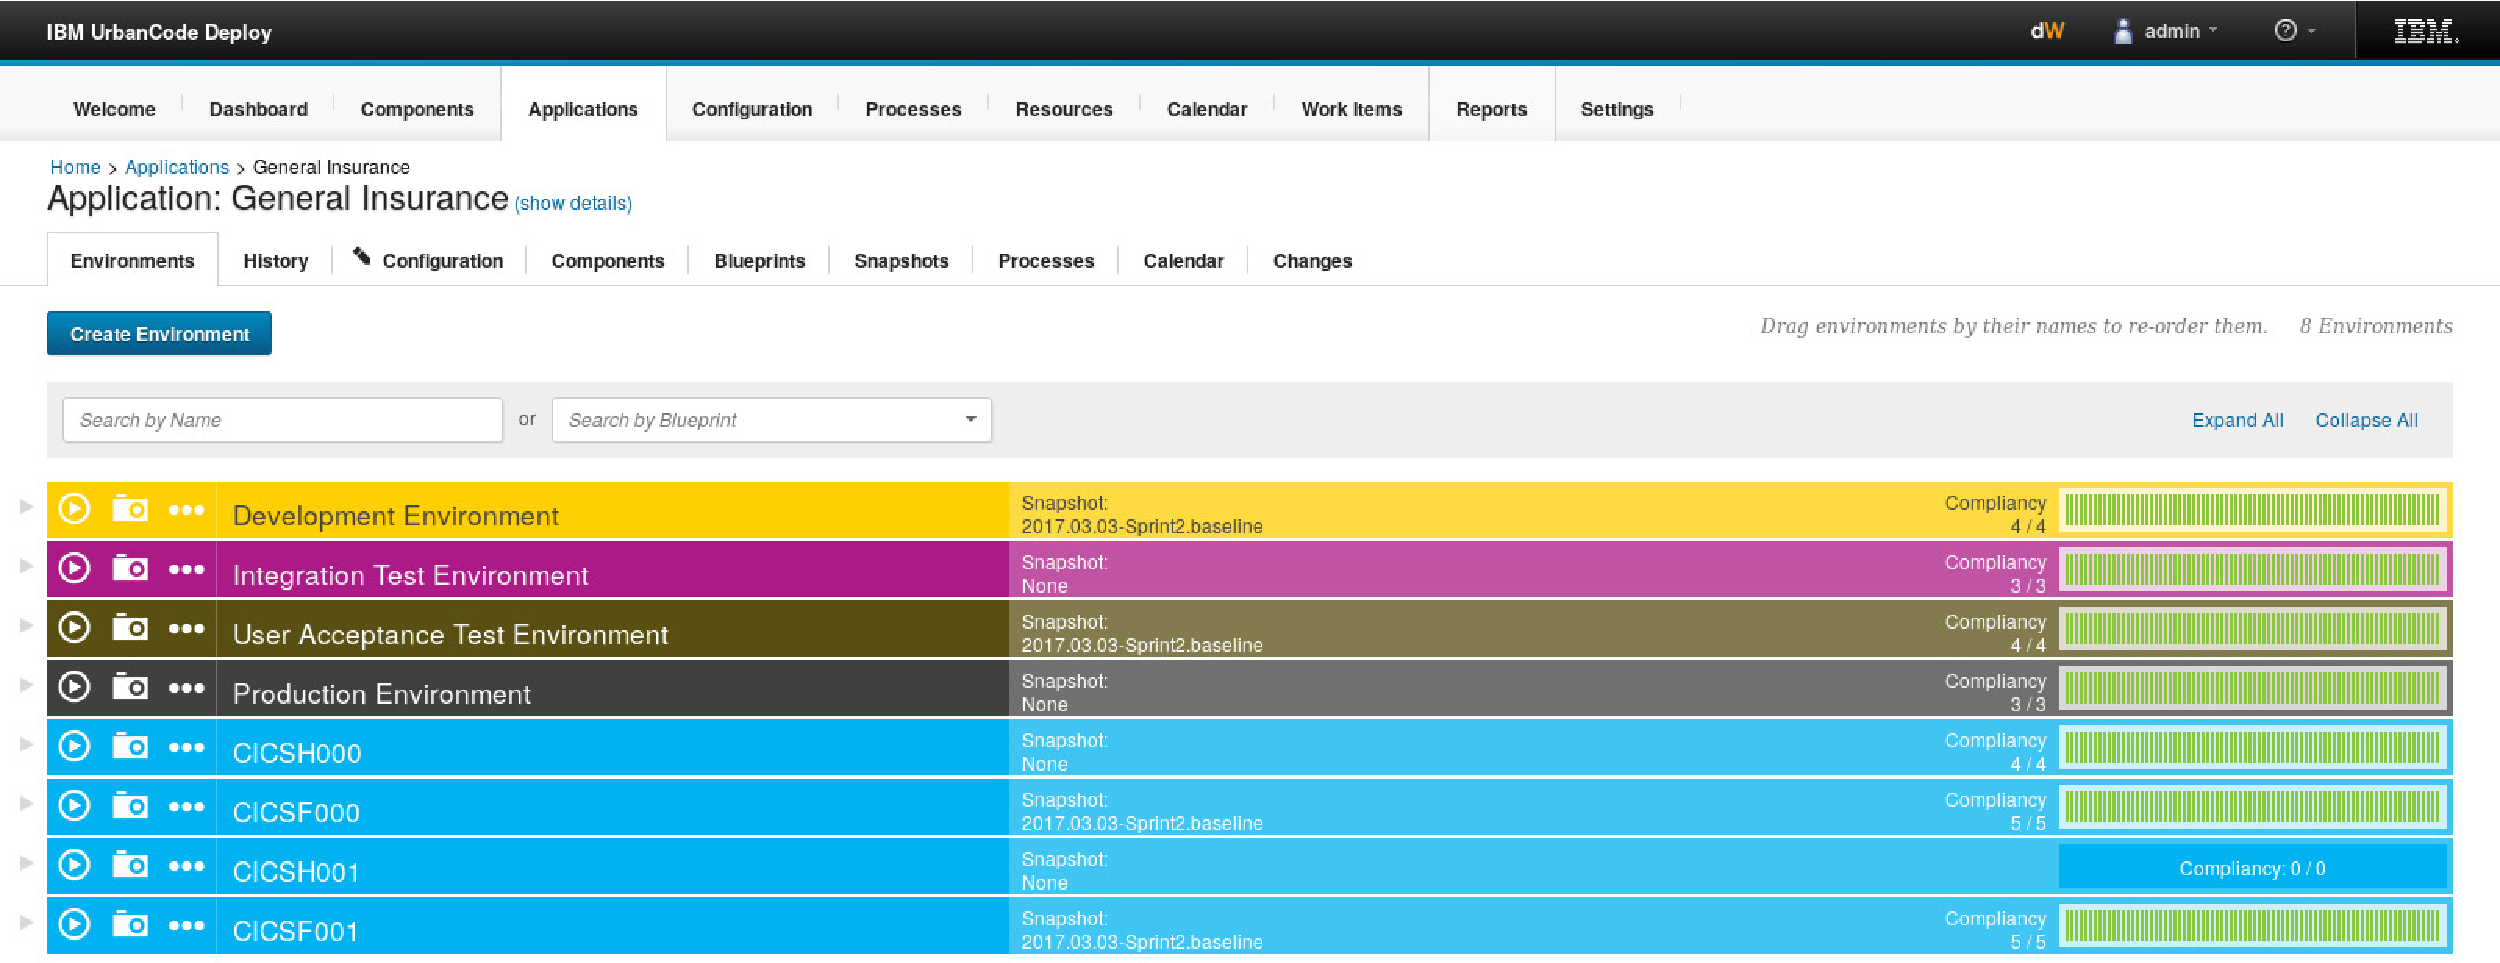
\includegraphics[scale=0.31]{images/kapitel_3/ucd_overview.pdf}
  \caption{Übersicht der Systeme in UCD}
  \label{fig:ucd_overview}
\end{figure}

Es muss lediglich eine Applikation im UCD eingerichtet werden. Die Einrichtung einer Anwendung in UCD ist relativ aufwendig
und kann im IBM Knowledge Center\footnote{https://ibm.co/2uSkr5M} nachgelesen werden. Dort wird die Einrichtung mit 2-3
Stunden angegeben.

Ist die Einrichtung allerdings erfolgreich fertiggestellt, kann, wie in Abbildung \ref{fig:ucd_start} auf Seite
\pageref{fig:ucd_start} zu sehen, eine CICS-Region mit der gewünschten Anwendung bestückt werden.

\begin{figure}[h]
  \centering
    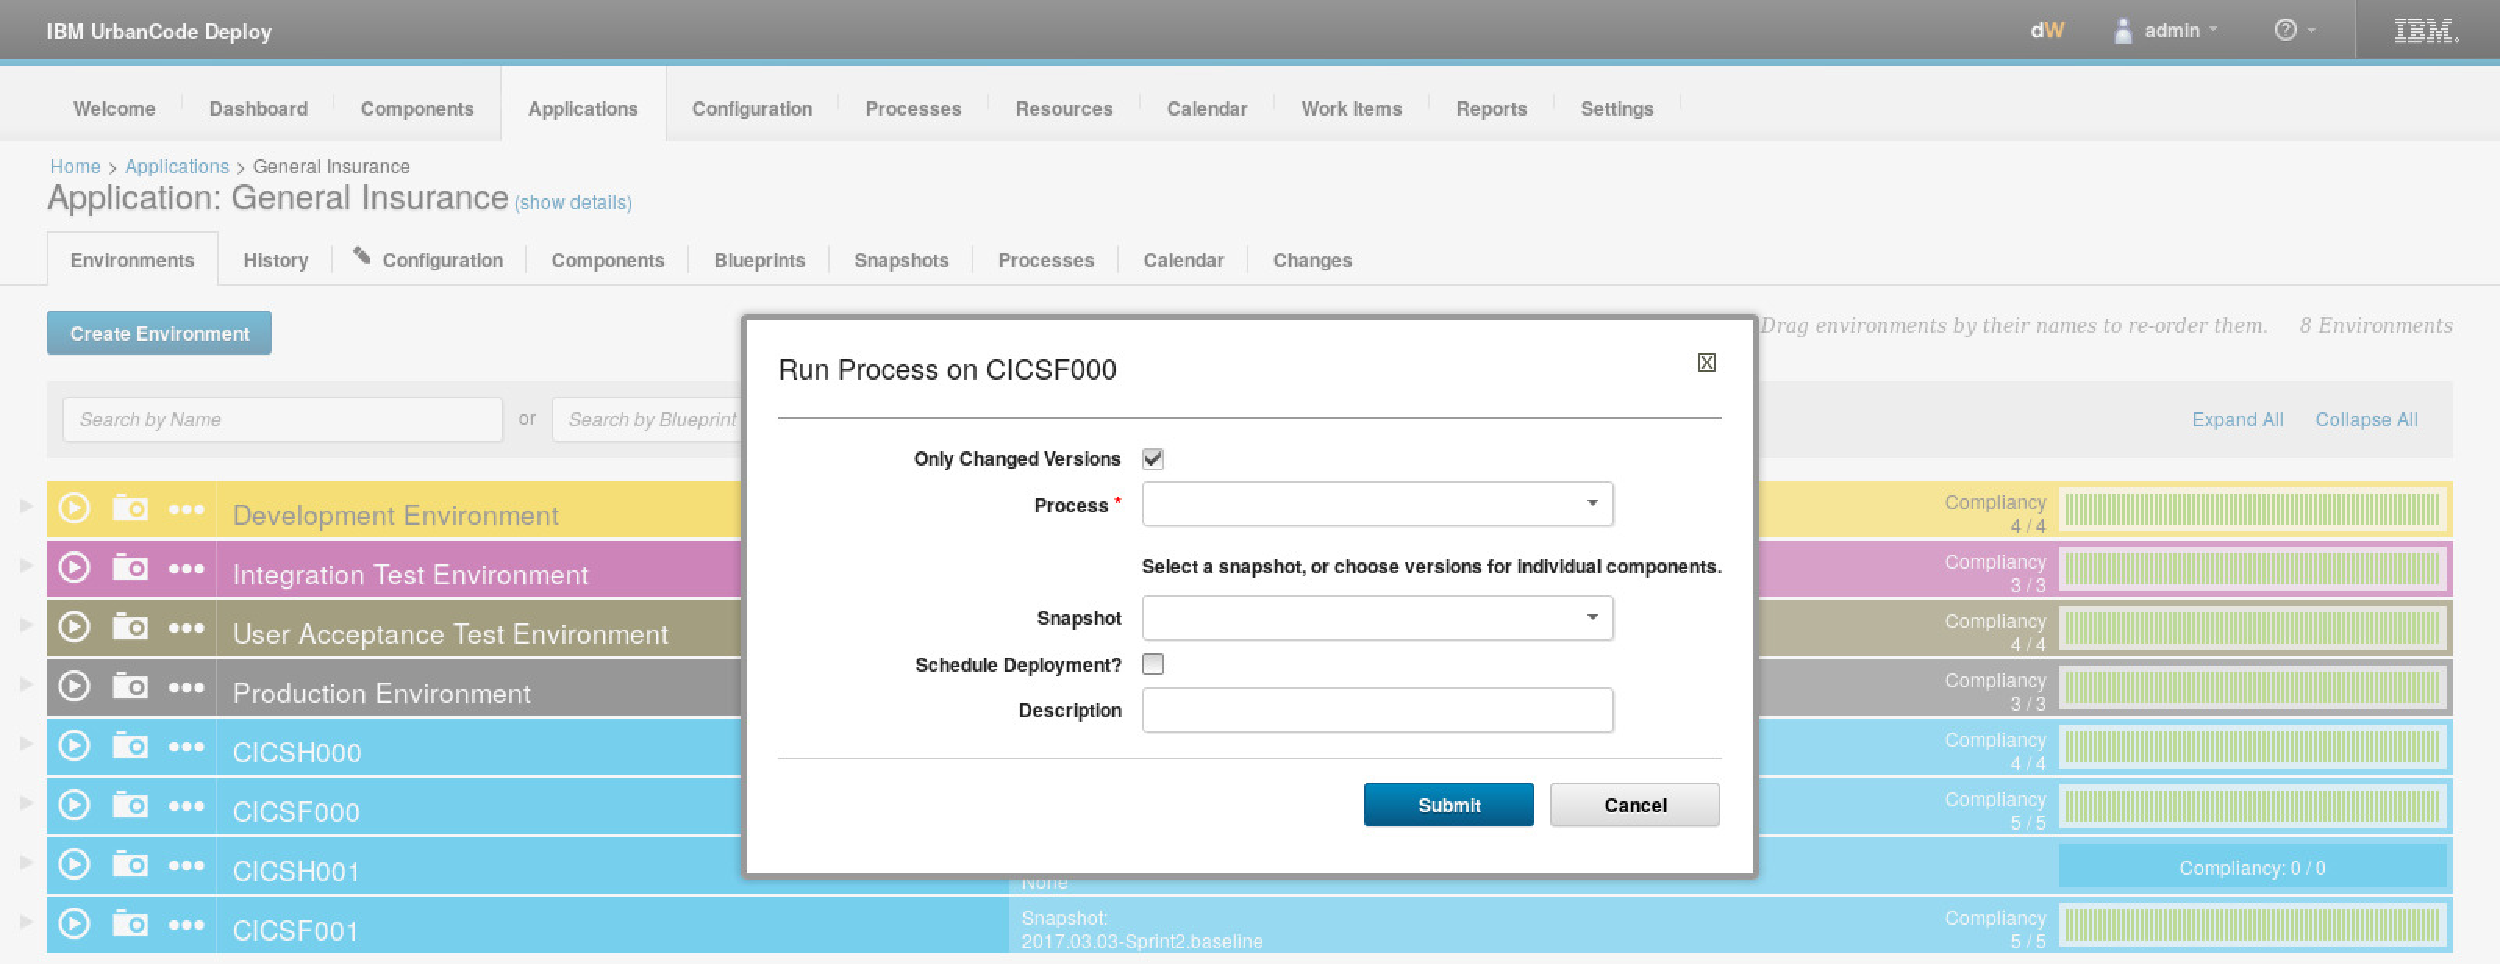
\includegraphics[scale=0.31]{images/kapitel_3/ucd_start.pdf}
  \caption{Start eines Deployments}
  \label{fig:ucd_start}
\end{figure}

Nach dem Start der Aufgabe sollte es lediglich wenige Minuten dauern, bis die Anwendung erfolgreich auf der ausgewählten
CICS-Region zur Verfügung steht.